\documentclass{article}
\usepackage[margin=1in]{geometry}
\usepackage{setspace}
\usepackage{graphicx}
\usepackage{amsmath}
\usepackage{booktabs}
\usepackage{multirow}
\usepackage[colorlinks=true,linkcolor=blue,citecolor=blue,urlcolor=blue]{hyperref}  % load last

\numberwithin{equation}{section}   % equations numbered (2.13), where "2" is the section number

\def\DS{{\rm DS}}
\def\DD{{\rm DD}}
\def\LAG{{\rm LAG}}
\def\nn{\nonumber}

\title{Notes on the ``pirate'' dedisperser (in progress)}
\author{Kendrick Smith}

\begin{document}

\maketitle

\tableofcontents

\setstretch{1.05}   % spacing between lines
\setlength{\parskip}{2.5pt}  % spacing between paragraphs

\clearpage

\section{Tree dedispersion}
\label{sec:tree_dedispersion_top}

\subsection{Tree gridding kernel}
\label{sec:gridding}

Our starting point for tree dedispersion is a shape $(N_{\rm freq}, N_{\rm time})$ array representing channelized intensity time series. We do not assume that frequency channels are evenly spaced (in CHORD we use unequal spacing).
We want to search this array for FRBs with delay $\propto \nu^{-2}$.

The first step is a ``tree gridding'' kernel which changes variables so that the delay is linear (i.e.~the FRB dispersion sweep looks like a straight line).
The input of the tree gridding kernel is a shape $(N_{\rm freq}, N_{\rm time})$ array, and the output is a shape $(N_{\rm tree}, N_{\rm time})$ array, where $N_{\rm tree}=2^r$.
The parameter $r$ is the tree dedispersion ``rank'' and is specified in a config file.

The leading axis of the input array represents frequency channels, and will be indexed by $0 \le F < N_{\rm freq}$.
The leading axis of the output array represents a reparameterized frequency channel (``tree-freq'' channel for short), and will be indexed by $0\le f < 2^r$.
Conceptually, the tree gridding kernel just reparameterizes the frequency axis (i.e.\ the time axis is a spectator.)

The tree gridding kernel also takes an auxiliary array \verb|channel_map|, which describes the mapping between frequency channels $0 \le F < N_{\rm freq}$ and tree-freq channels $0 \le f < N_{\rm tree}$.
The array \verb|channel_map| has length $N_{\rm tree}+1$, and its entries are (in general non-integer) frequency-channel indices in the range $[0, N_{\rm freq}]$.
Writing $c_f$ for the $f$-th entry, tree-freq channel $f$ is defined to occupy the half-open interval of frequency channels
\begin{equation}
I_f = \big[\, c_{f+1},\ c_f \,\big), \qquad 0 \le f < N_{\rm tree},
\end{equation}
i.e.~consecutive entries give the lower and upper edges of each tree-freq channel.
The entries are fixed by the dispersion geometry: the tree-freq channels are equally spaced in the dispersion variable $x \equiv \nu^{-2}$ (this is the change of variables that linearizes the delay), so the $f$-th edge sits at
\begin{equation}
x_f = \nu_{\rm hi}^{-2} + \frac{f}{N_{\rm tree}}\left(\nu_{\rm lo}^{-2} - \nu_{\rm hi}^{-2}\right),
\end{equation}
and $c_f$ is the frequency-channel index of the frequency $\nu_f = x_f^{-1/2}$, where the index increases with frequency, running from $0$ at the band bottom $\nu_{\rm lo}$ to $N_{\rm freq}$ at the band top $\nu_{\rm hi}$.
In particular $c_0 = N_{\rm freq}$ and $c_{N_{\rm tree}} = 0$, so \verb|channel_map| is monotonically {\em decreasing} ($c_{f+1} < c_f$).
We store it in double precision, since the gridding weights below are obtained by differencing adjacent entries, which loses relative precision.

The details of the tree gridding kernel are as follows.
Each output tree-freq channel $f$ is a weighted sum of the input frequency channels whose bins overlap the interval $I_f = [c_{f+1}, c_f)$:
\begin{equation}
{\rm out}[f] = \sum_{F=0}^{N_{\rm freq}-1} w_{fF}\, {\rm in}[F],
\end{equation}
where ${\rm in}[F]$ and ${\rm out}[f]$ are length-$N_{\rm time}$ time series, and the same weights are applied at every time sample (the time axis is untouched).
The weight $w_{fF}$ is the length of the overlap between the tree-freq channel interval $I_f$ and the unit-width frequency bin $[F, F+1)$:
\begin{equation}
w_{fF} = \max\!\big(\,0,\ \min(c_f,\, F+1) - \max(c_{f+1},\, F)\,\big).
\end{equation}
A frequency channel lying entirely within $I_f$ contributes with weight $1$, while a channel straddling an edge of $I_f$ contributes a fractional weight.
Because the intervals $I_f$ tile $[0, N_{\rm freq}]$, the weights of any fixed input channel sum to one, $\sum_f w_{fF} = 1$; the gridding kernel is thus a delay-linearizing rebinning of the frequency axis that conserves total intensity, $\sum_f {\rm out}[f] = \sum_F {\rm in}[F]$.

Note that the tree gridding kernel is a monotone {\em decreasing} reindexing operation.
Thus, to search for FRBs with positive dispersion (lowest frequencies arise last), we want to search over lines in the tree array with positive slope (highest tree-freq channels arrive last).

\subsection{Tree dedispersion}
\label{sec:tree_dedispersion}

After the tree gridding kernel, the next step is ``tree dedispersion'', which searches for straight lines with $0\le \mbox{slope} \le 1$.
(The extension to slope $>1$ will be discussed in a future section, along with more details such as subband searches, early triggers, and peak-finding.)

The dedispersion input array has shape $(2^r, N_{\rm time})$, where the leading axis is ``tree-freq'' (see above).
Straight lines will be parameterized by an integer $0 \le d < 2^r$, representing
the delay (in time samples) between the lowest and highest tree-freq channel,
and a time index $t$ representing the arrival time in the {\em highest} tree-freq channel
(i.e. the {\em latest} arrival time).
Thus, the dedispersion output array also has shape $(2^r, N_{\rm time})$, where the first axis represents a delay (or DM).\footnote{Frequently in the code (but not in these notes), it's convenient to use a {\em bit-reversed} delay index $0 \le d_{\rm rev} < 2^r$. (This turns out to allow some array operations to operate ``in place'', facilitating parallelization.)}

Tree dedispersion is a composition of functions:
\begin{equation}
\big( \mbox{Input array} \big)
  \overset{\DS(0)}{\longrightarrow} \big( \mbox{Intermediate array} \big)
  \overset{\DS(1)}{\longrightarrow} \cdots 
  \overset{\DS(r-1)}{\longrightarrow}
\big( \mbox{Output array} \big)
\label{eq:DD_composition}
\end{equation}
where the function $\DS(k)$ (``dedispersion step $k$'') is described as follows:

\begin{itemize}

\item
The $\DS(k)$ input array is a shape $(2^{r-k}, 2^k, N_{\rm time})$ array.
The first axis represents a coarse frequency channel.
Each coarse-freq channel $f$ corresponds to a block of $2^k$ tree-freq channels
in the original tree input array:
\begin{equation}
2^k \, f \le (\mbox{tree-freq index}) < 2^k (f+1)  \label{eq:coarse_freq}
\end{equation}
The second axis represents a delay $0 \le d < 2^k$ within the coarse-freq channel
(\ref{eq:coarse_freq}). As $k$ increases, the coarse-freq channels double in width,
and we need twice as many delay indices to cover the range $0 \le (\mbox{slope}) \le 1$.

The time index represents an arrival time at the largest tree-freq channel
in the coarse-freq channel (\ref{eq:coarse_freq}), i.e.~the latest arrival time within the coarse-freq channel.

\item The $\DS(k)$ operation is defined by:

\begin{align}
{\tt out}[f,2d,t] &= \frac{1}{\sqrt{2}} 
  \big( {\tt in}[2f,d,t-d] + {\tt in}[2f+1,d,t] \big) \nn \\
{\tt out}[f,2d+1,t] &= \frac{1}{\sqrt{2}} 
  \big( {\tt in}[2f,d,t-d-1] + {\tt in}[2f+1,d,t] \big)
\end{align}

\item
As formulated above, tree dedispersion can lead to negative time indices.
By default, \verb|in[...,t]| with $t<0$ is defined to be zero.
(In the real-time system, we run tree dedispersion in an ``incremental'' context where a negative time index should be interpreted as a reference to data received in a previous time chunk.)

\item The $\DS(0)$ input array is sometimes reshaped from $(2^r,1,N_{\rm time})$
 to $(2^r,N_{\rm time})$, and the $\DS(r-1)$ output array is sometimes reshaped
 from $(1,2^r,N_{\rm time})$ to $(2^r,N_{\rm time})$.
 Thus, we think of the entire tree dedispersion operation (\ref{eq:DD_composition}) as having input and output shapes $(2^r, N_{\rm time})$.

\end{itemize}

\par\noindent
We define $\DD(r)$ (``rank-$r$ dedispersion'') to be the composition of all $r$ steps in Eq.\ (\ref{eq:DD_composition}):
\begin{equation}
\DD(r) = \DS(r-1) \circ \cdots \circ \DS(0)  \label{eq:DD_DS}
\end{equation}

\subsection{Subband search}
\label{sec:subband_search}

So far, we have described a search for FRBs which cover the full tree-freq range $0 \le f < 2^r$.
This would be suboptimal since real FRBs do not always cover the full frequency range.
Next, we introduce a ``sub-band'' search for searching a configurable set of subbands.

\subsubsection{Parameterization of subbands}

Our dedispersion config files contain a length-$(R+1)$ integer-valued array of subband counts $C_l$.\footnote{In 
the code, $R$ is denoted {\tt pf\_rank}, $l$ is denoted {\tt pf\_level}, and $C_l$ is denoted {\tt frequency\_subband\_counts}.}
Here $0 \le R \le r$, where $r$ is the tree rank.
The counts $C_l$ parameterize a set of subbands as follows:
\begin{itemize}
\item Frequency subbands are indexed by a pair $(l,s)$ where $0 \le l \le R$ and $0 \le s < C_l$.
We will sometimes ``flatten'' the pair $(l,s)$ into a single subband index $0 \le n < N$, where
\begin{equation}
N \equiv \sum_{l=0}^R C_l
\end{equation}
is the total number of subbands. 
(In the code, $n$ and $N$ are denoted by the same symbols, e.g.\ $N$ is {\tt FrequencySubbands::N}.)
\item Level $l=0$ is special: subband $(0,s)$ corresponds to tree-freq range
\begin{equation}
2^{r-R} s \le \mbox{(tree-freq index)} < 2^{r-R} (s+1)  \label{eq:subband_l0}
\end{equation}
\item At levels $l>0$, subband $(l,s)$ corresponds to tree-freq range
\begin{equation}
2^{r-R+l-1} s \le \mbox{(tree-freq index)} < 2^{r-R+l-1} (s+2)  \label{eq:subband_l1}
\end{equation}
Thus, level 0 consists of non-overlapping bands whose fractional width is $1/2^R$.
Levels $l>0$ consist of bands whose fractional width is $1/2^{R-l}$, and overlap by a factor 2.
\item
To avoid ``overflowing'' the band, $C_l$ must satisfy
\begin{equation}
0 \le C_l \le \begin{cases}
2^R & \mbox{for } l=0 \\
2^{R-l+1}-1 & \mbox{for } l>0
\end{cases}
\end{equation}
A level with $C_l=0$ is allowed, and simply contributes no subbands.
We require $C_R=1$, i.e.~we always search the full frequency band.
The case $C_l=\{1\}$ (with $R=0$) corresponds to disabling subbands, and only searching the full band.
\item The details of this scheme, including the ``specialness'' of level $l=0$, are
dictated by convenience in the GPU kernel.
\item To {\em interpret} the $C_l$ already in a config file, run \verb|pirate_frb show_dedisperser -cv|.
For example, for $C_l=[5,9,7,3,1]$ this prints:
\begin{verbatim}
# In this config, there are 25 top-level frequency subband(s):
#   pf_level=0: [948.7,1500.0], [750.0,948.7], [639.6,750.0], [566.9,639.6], [514.5,566.9]
#   pf_level=1: [750.0,1500.0], [639.6,948.7], [566.9,750.0], [514.5,639.6], [474.3,566.9],
#               [442.3,514.5], [416.0,474.3], [393.9,442.3], [375.0,416.0]
#   pf_level=2: [566.9,1500.0], [474.3,750.0], [416.0,566.9], [375.0,474.3], [344.1,416.0],
#               [319.8,375.0], [300.0,344.1]
#   pf_level=3: [416.0,1500.0], [344.1,566.9], [300.0,416.0]
#   pf_level=4: [300.0,1500.0]
\end{verbatim}
\item To {\em create} a $C_l$ array with a given max $\Delta(\log \nu)$, run \verb|pirate_frb make_subbands|.
For example, \verb|pirate_frb make_subbands 300 1500 0.1 -r 4| gives $C_l=[5,9,7,3,1]$.
These subbands are shown visually in Figure \ref{fig:subbands}.
\end{itemize}
\begin{figure}
\centering
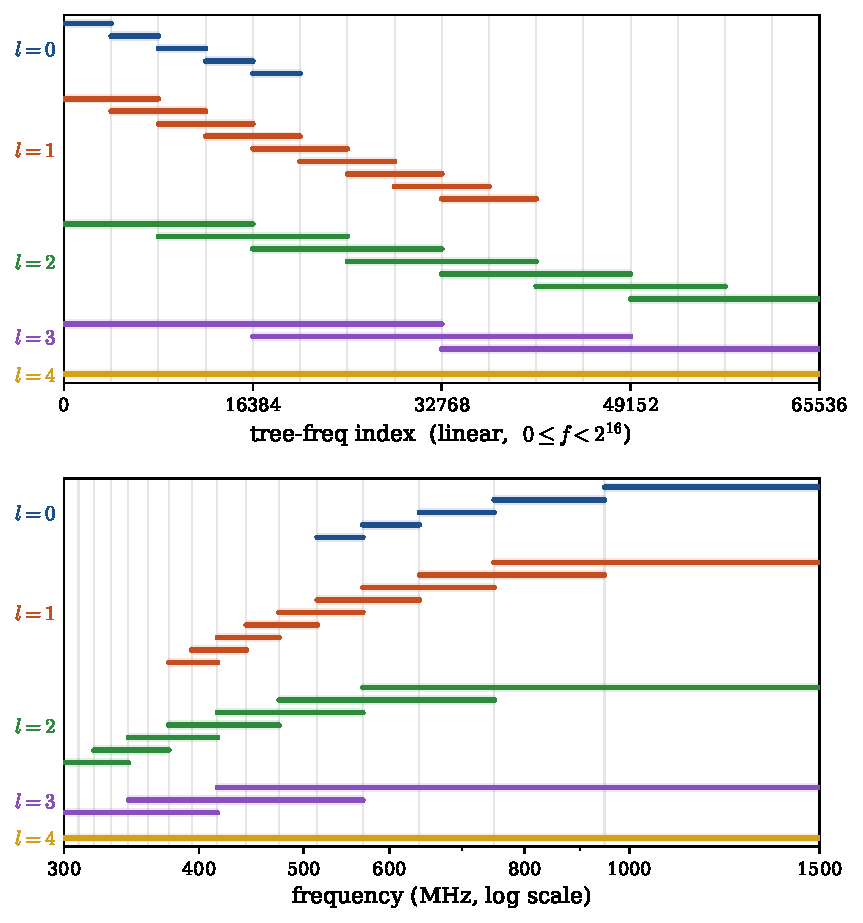
\includegraphics[width=\textwidth]{figs/chord_subbands.pdf}
\caption{Frequency subbands in a CHORD config with {\tt frequency\_subband\_counts=[5,9,7,3,1]}).
The top panel shows the subbands in tree-freqs (where they are ``naturally'' defined) and the bottom
panel shows the conversion to physical frequency $\nu$ in MHz. Note that the conversion between tree-freqs
and $\nu$ is monotone decreasing.}
\label{fig:subbands}
\end{figure}

\subsubsection{Subbanded dedispersion}

Subbanded dedispersion is an operation whose input array is the same as ordinary (non-subbanded) tree 
dedispersion (\ref{sec:tree_dedispersion}), i.e.\ a shape $(2^r, N_{\rm time})$ array where the first index is tree-freq.
The output array has shape $(2^{r-R}, M, N_{\rm time})$, where $M$ is the number of ``multiplets'':
\begin{equation}
M \equiv \sum_{l=0}^R 2^l C_l  \label{eq:multiplet_def}
\end{equation}
Each subband $(l,s)$ ``owns'' a shape $(2^{r-R}, 2^l, N_{\rm time})$ subarray of the output.
The first two axes correspond to $2^{r-R+l}$ dispersion delays across the subband, split into a ``coarse'' index
$0 \le d_{\rm hi} < 2^{r-R}$ and a ``fine'' index  $0 \le d_{\rm lo} < 2^l$.
(This index-splitting ensures that the combined output of all subbands is a regular $(2^{r-R}, M, N_{\rm time})$ array,
rather than a ``ragged'' object.)

Conceptually, subband dedispersion works as follows.
For each subband $(l,s)$, we apply tree dedispersion to the appropriate tree-freq range (either Eq.\ (\ref{eq:subband_l0}) 
or (\ref{eq:subband_l1})). We also apply a time lag so that the time index corresponds to the extrapolated arrival time at 
the highest tree-freq in the full band, not the highest tree-freq in the subband.
For an efficient implementation, we run tree dedispersion as usual (Eq.\ \ref{eq:DD_composition}), and extract per-subband
dedispersion outputs from intermediate arrays ``on the fly'', rather than dedispersing each subband ``from scratch''.

Formally, the details are as follows:

\begin{itemize}

\item {\bf Case 1: $l=0$ or even $s$.}
In this case, the subband corresponds to an ``aligned'' tree-freq range of the form:
\begin{equation}
2^{r-R+l} f \le \mbox{(tree-freq index)} < 2^{r-R+l}(f+1) \hspace{1cm} \mbox{(where $0 \le f < 2^{R-l}$)}
\end{equation}
where the coarse-freq index $f$ is given by:
\begin{equation}
f = \begin{cases} s & \mbox{if } l=0 \\ s/2 & \mbox{if } l > 0 \end{cases}
\end{equation}
The subband owns a shape $(2^{r-R}, 2^l, N_{\rm time})$ subarray of the output (denote by \verb|out|).

In this case, the per-subband dedispersion outputs already arise as intermediates in tree dedispersion
(Eq.\ \ref{eq:DD_composition}); we just need to apply a time lag.
Let \verb|tmp| be the output array of $\DS(k-1)$, where $k=r-R+l$. 
Then \verb|tmp| has shape $(2^{R-l}, 2^{r-R+l}, N_{\rm time})$.
To populate the \verb|out| array, we slice/reshape \verb|tmp| and apply time lags:
\begin{equation}
{\tt out}\big[ d_{\rm hi}, d_{\rm lo}, t \big] = {\tt tmp}\big[ f, d, t - T \big]
\end{equation}
where on the RHS we define:
\begin{equation}
d \equiv d_{\rm hi} 2^l + d_{\rm lo}   \hspace{1.5cm} T \equiv d_{\rm hi} 2^l (2^{R-l}-1-f)
\end{equation}

\item {\bf Case 2: $l>0$ and odd $s$.}
In this case, the subband corresponds to a ``half-aligned'' tree-freq range of the form:
\begin{equation}
2^{r-R+l-1} (2f+1) \le \mbox{(tree-freq index)} < 2^{r-R+l-1}(2f+3) \hspace{1cm} \mbox{(where $0 \le f < 2^{R-l}-1$)}
\end{equation}
where the coarse-freq index $f$ is given by $f \equiv (s-1)/2$.
The subband owns a shape $(2^{r-R}, 2^l, N_{\rm time})$ subarray of the output (denote by \verb|out|).

This case is a little more complicated, since the per-subband dedispersion outputs are ``one dedispersion step away''
from the intermediate arrays in tree dedispersion.
Let \verb|tmp| be the output array of $\DS(k-1)$, where $k=r-R+l-1$. 
Then \verb|tmp| has shape $(2^{R-l+1}, 2^{r-R+l-1}, N_{\rm time})$.
\begin{align}
{\tt out}\big[ d_{\rm hi}, 2 d_{\rm lo}, t \big] 
  &= \frac{1}{\sqrt{2}} \Big( {\tt tmp}\big[ 2f+1, d, t - T_0 - d \big] + {\tt tmp}\big[ 2f+2, d, t - T_0 \big] \Big) \nn \\
{\tt out}\big[ d_{\rm hi}, 2 d_{\rm lo} + 1, t \big] 
  &= \frac{1}{\sqrt{2}} \Big( {\tt tmp}\big[ 2f+1, d, t - T_1 - d - 1 \big] + {\tt tmp}\big[ 2f+2, d, t - T_1 \big] \Big) 
\end{align}
where on the RHS we define:
\begin{equation}
d \equiv d_{\rm hi} 2^{l-1} + d_{\rm lo}
  \hspace{1.5cm} T_0 = T_1 = d_{\rm hi} 2^{l-1} (2^{R-l+1} - 2f - 3)
\end{equation}
(Warning: the quantities $f,k,d_{\rm lo}$ have slightly different meanings in cases 1 and 2!)

\end{itemize}
Note that subband dedispersion includes the full band (via $C_R=1$), but the full-band output array is
``reshaped'' to $(2^{r-R}, 2^R, N_{\rm time})$, whereas in the previous section it had shape $(2^r, N_{\rm time})$.

\medskip
\noindent{\bf Remark (time-lag convention).}
The lags $T$ (Case 1) and $T_0 = T_1$ (Case 2) above depend only on the {\em coarse} delay $d_{\rm hi}$,
not on the fine delay $d_{\rm lo}$: both equal $g\, d_{\rm hi}$, where $g$ is the number of coarse
channels (each $2^{r-R}$ tree-freq channels wide) lying above the subband.
Equivalently, the $2^l$ fine-DM multiplets that share a given subband and coarse delay $d_{\rm hi}$ are
assigned a {\em common} time origin, extrapolated to the full-band top from the coarse delay alone.
This is the convention used by the GPU kernel and \verb|ReferenceTree| (their \verb|ff*dd|), and we
adopt it here only to match the current code.

Arguably it would make more sense to reference each multiplet to the full-band-top arrival
extrapolated from its {\em own} (full) subband delay, so that a given burst peaks at the same output
time index for every multiplet of its DM. That choice replaces the lags above by
\begin{align}
\mbox{Case 1:}\quad & T = d\,(2^{R-l}-1-f), \qquad\quad d = d_{\rm hi}2^l + d_{\rm lo}, \nn \\
\mbox{Case 2:}\quad & T_0 = d\,(2^{R-l+1}-2f-3), \qquad T_1 = T_0 + (2^{R-l}-f-2),
\end{align}
i.e.~the (floored) half-integer extrapolation, for which $T_0 \ne T_1$. We may switch the code to
this convention in the future.

\subsection{Peak-finding}
\label{sec:peak_finding}

The final stage of the dedispersion transform is {\em peak-finding}.
For now, we give a partial description -- a future version of the notes will describe
peak-finding in more detail.
The input is the shape-$(2^{r-R}, M, N_{\rm time})$ array from the previous section.
The output is a shape-$(2^{r-R}, N_{\rm time}/T_{\rm ds})$ array, where $T_{\rm ds}$ is a time downsampling factor.
Conceptually, peak-finding is 3 steps:
\begin{itemize}
\item For each $(d_{\rm hi}, m)$, the input array is a 1-d time series.
We convolve the time series with $P$ peak-finding kernels, described below, to
obtain a shape $(2^{r-R}, M, N_{\rm time}, P)$ array.
\item We apply weights that depend on $(d_{\rm hi}, m, p)$, to normalize the array 
so that each array element has variance 1. (Thus, array elements are normalized to
``sigmas''.)
\item We downsample the array to shape $(2^{r-R}, N_{\rm time}/T_{\rm ds})$.
Downsampling is done with ``max'' rather than addition, so each array element
corresponds to max detection significance over all downsampled parameters.
\end{itemize}
In implementation, these 3 steps are coalesced into one GPU kernel for speed (and also
coalesced with the final stages of tree dedispersion), e.g.\ the shape $(2^{r-R}, M, N_{\rm time}, P)$
is never ``materialized'' in GPU memory.

\subsubsection{Peak-finding kernels}

The kernels are organized into $\Lambda \equiv \max(\log_2 W_{\rm max},\,1)$ {\em levels} $0 \le \lambda < \Lambda$,\footnote{In the code these are denoted {\tt l} and {\tt L}; we use $\lambda$ and $\Lambda$ here to avoid ambiguity with the subband level $l$ in \S\ref{sec:subband_search}.} where
$W_{\rm max}$ (a power of two) is the config parameter \verb|max_kernel_width|. The total number of
profiles is
\begin{equation}
P = 3 \log_2 W_{\rm max} + 1.
\end{equation}
The building block at level $\lambda$ is the {\em unnormalized running boxcar sum} of width $2^\lambda$,
\begin{equation}
b_\lambda[t] \equiv \sum_{i=0}^{2^\lambda - 1} x[t-i],
\end{equation}
computed by the recursion
\begin{equation}
b_0[t] = x[t], \qquad b_{\lambda+1}[t] = b_\lambda[t] + b_\lambda[t - 2^\lambda].
\label{eq:boxcar_recursion}
\end{equation}
Note that (\ref{eq:boxcar_recursion}) is a {\em plain sum}: there is no $1/\sqrt2$ in the boxcar
downsampling. (All normalization is deferred to the weights.)

At each level $\lambda$ we form up to four kernels, denoted $h_{\lambda,q}$ where $0\le q \le 3$:
\begin{align}
h_{\lambda,0} &= [\,\underbrace{1,\dots,1}_{2^\lambda}\,] \nn \\
h_{\lambda,1} &= [\,\underbrace{1,\dots,\dots,1}_{2^{\lambda+1}}\,] \nn \\
h_{\lambda,2} &= [\,\underbrace{\tfrac12,\dots}_{2^\lambda},\ \underbrace{1,\dots}_{2^\lambda},\ \underbrace{\tfrac12,\dots}_{2^\lambda}\,] \nn \\
h_{\lambda,3} &= [\,\underbrace{\tfrac12,\dots}_{2^\lambda},\ \underbrace{1,\dots,\dots,1}_{2^{\lambda+1}},\ \underbrace{\tfrac12,\dots}_{2^\lambda}\,]
\end{align}
The profile index $0\le p < P$ is related to $(\lambda,q)$ by $p = 3\lambda + q$, with the special value $p = 0$ for
$(\lambda,q) = (0,0)$. Thus level $0$ contributes profiles $p = 0,1,2,3$, and each level $\lambda > 0$ contributes
$p = 3\lambda+1, 3\lambda+2, 3\lambda+3$ --- the single-boxcar kernel $h_{\lambda,0}$ is dropped for $\lambda>0$, since
$h_{\lambda,0} = b_\lambda = h_{\lambda-1,1}$ would be redundant.

\subsection{Time-downsampled trees and early triggers}
\label{sec:downsampled_early}

So far, we have described a single {\tt DedispersionTree} which searches up to slope 1 (i.e.~full-band dispersion delay equal to $2^r$ time samples), and ``triggers'' when the pulse arrives at the lowest frequency (highest tree-freq).
It will be useful to define a larger {\tt Dedisperser} object, consisting of multiple trees, as follows:

\begin{itemize}

\item {\bf Downsampled trees} in order to search to higher DM. 
If we time-downsample the data by a factor $2^p$, and run rank-$r$ dedispersion as usual, then we can search to a max dispersion delay which is larger by a factor $2^p$.
When we time-downsample by a factor $2^p$, we add time samples and multiply by $2^{-p/2}$, in order to leave the variance unchanged (assuming uncorrelated samples).

If $p > 0$, then we only keep the upper half (in delay) of the dedispersion output, since the lower half was already searched by primary tree $(p-1)$.
Thus, each value of $p$ corresponds to a different DM range, ordered from low to high DM.

\item {\bf Early triggers} in order to reduce triggering latency, especially at high DM. 
By default, we only trigger when the pulse arrives at the highest tree-freq $f=2^r$ (i.e.\ lowest radio frequency).
If we run parallel tree dedispersion over the lowest $2^{r-e}$ tree-freqs (i.e.\ highest radio frequencies),
then the triggering time will be smaller by a factor $2^e$.
This comes at the expense of losing low frequencies, so not all bursts will be detected in the early trigger.

\end{itemize}

\par\noindent
The {\tt Dedisperser} consists of multiple trees parameterized by $(p,e)$.
In the dedispersion config file, the syntax is (from {\tt chord\_sb2\_et.yml}):
\begin{verbatim}
  toplevel_tree_rank: 16    # rank r of "top-level" tree (p=0, e=0)

  primary_trees:
    - {num_early_triggers: 0, ...}   # This line creates one tree with p=0, e=0
    - {num_early_triggers: 1, ...}   # This line creates two trees with p=1, e=0,1
    - {num_early_triggers: 2, ...}   # This line creates three trees with p=2, e=0,1,2
    - {num_early_triggers: 3, ...}   # This line creates four trees with p=3, e=0,1,2,3
\end{verbatim}
In the code, data structures are as follows:
\begin{itemize}
\item There is one ``top-level'' tree with $p=e=0$ (no time downsampling, no early triggers) and rank $r = {\tt toplevel\_tree\_rank}$.
\item There are four ``primary'' trees with $e=0$ (no early triggers) and $p=0,1,2,3$.
Each primary tree searches a different DM range, ordered from low to high DM.
\item Each primary tree corresponds to multiple {\tt DedispersionTrees} with $0 \le e \le {\tt num\_early\_triggers}$.
These trees (for fixed $p$) search the same DM range, with different threshold frequencies for triggering, ordered from latest in time (lowest frequency) to earliest (highest frequency).
\end{itemize}
The integer $p$ is called the {\em primary tree index}, and the integer $e$ is called the {\em early trigger level}.
Conceptually, each {\tt DedispersionTree} just runs ``vanilla'' rank-$(r-e$) tree dedispersion on the first $2^{r-e}$ tree-freqs, downsampled in time by $2^p$, and then drops the lower DM-half of the outputs if $p > 0$.\footnote{This description suggests that each tree is an independent computation run ``from scratch''. There are a lot of tricks in the code that reuse computations between trees, i.e.\ the {\tt Dedisperser} is faster than running the constituent {\tt DedispersionTrees} independently.}
For a more intuitive presentation of these trees, see Tab.\ \ref{tab:chord_sb2_et} and Figs.\ \ref{fig:early_triggers}, \ref{fig:tree_segments}.

\begin{table}[ht]
\centering
\begin{tabular}{c c c c c c}
\toprule
$p$ & $e$ & Full-band delay range (s) & DM range (pc\,cm$^{-3}$) & trigger (MHz) & latency range (s) \\
\midrule
0 & 0 & 0.0--65.5 & 0--1481 & 300 & 0.0--65.5 \\
\midrule
\multirow{2}{*}{1} & 0 & \multirow{2}{*}{65.5--131.1} & \multirow{2}{*}{1481--2962} & 300 & 65.5--131.1 \\
 & 1 & & & 416 & 32.8--65.5 \\
\midrule
\multirow{3}{*}{2} & 0 & \multirow{3}{*}{131.1--262.1} & \multirow{3}{*}{2962--5924} & 300 & 131.1--262.1 \\
 & 1 & & & 416 & 65.5--131.1 \\
 & 2 & & & 567 & 32.8--65.5 \\
\midrule
\multirow{4}{*}{3} & 0 & \multirow{4}{*}{262.1--524.3} & \multirow{4}{*}{5924--11847} & 300 & 262.1--524.3 \\
 & 1 & & & 416 & 131.1--262.1 \\
 & 2 & & & 567 & 65.5--131.1 \\
 & 3 & & & 750 & 32.8--65.5 \\
\bottomrule
\end{tabular}
\caption{The ten {\tt DedispersionTree}s of the CHORD config {\tt chord\_sb2\_et.yml} (rank $r=16$; four primary trees). Each tree is identified by a $(p, e)$ pair. The DM range and {\em full-band} dispersion delay range depend only on $p$. The trigger frequency depends only on $e$, and the latency range is $2^{-e} \times \mbox{(delay range)}$.
(Generated with {\tt pirate\_frb show\_dedisperser -v configs/dedispersion/chord\_sb2\_et.yml}.)}
\label{tab:chord_sb2_et}
\end{table}

\begin{figure}[ht]
\centering
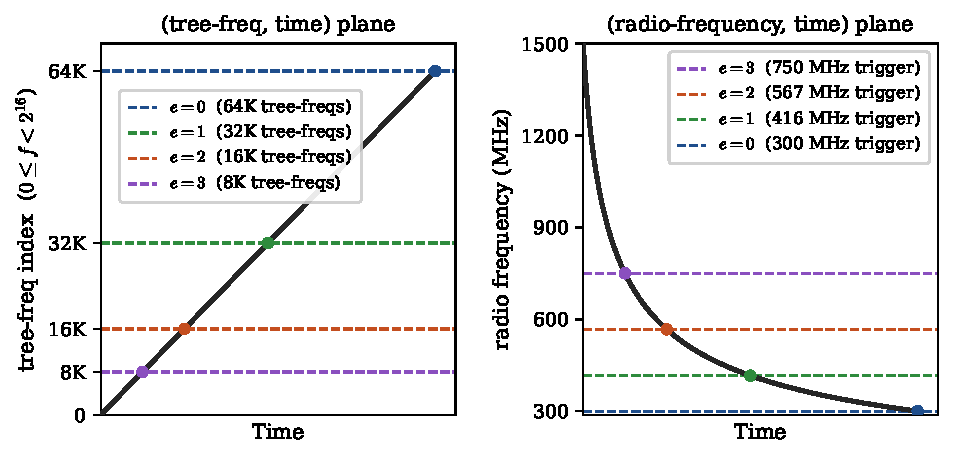
\includegraphics[width=\textwidth]{figs/early_triggers.pdf}
\caption{A visualization of early triggers, in radio frequency (right panel) or the ``tree-freq'' reparametrization used in the code (left panel). Trees with early triggers search the lower part of the tree-freq range, i.e.\ the high part of the radio frequency range. A tree with $e > 0$ triggers earlier (by a factor $2^e$) than the main tree. The plot assumes CHORD params (300--1500 MHz, $r=16$, $0\le e\le 3$).}
\label{fig:early_triggers}
\end{figure}

\begin{figure}[ht]
\centering
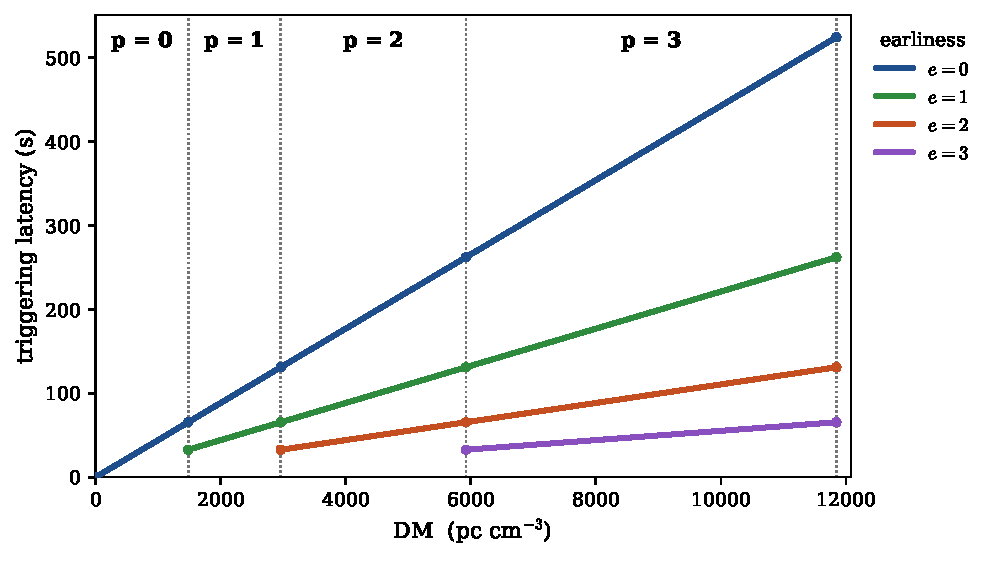
\includegraphics[width=0.85\textwidth]{figs/tree_segments.pdf}
\caption{The ten {\tt DedispersionTrees} from Table\ \ref{tab:chord_sb2_et}, shown as line segments in the (DM, triggering latency) plane. For each tree $(p, e)$, the value of $p$ determines the DM range, and the value of $e$ determines the slope.}
\label{fig:tree_segments}
\end{figure}

\clearpage

\subsection{Dedispersion output arrays}

The dedispersion output consists of a pair of 2-d arrays (\verb|out_max|, \verb|out_argmax|)
for each beam and \verb|DedispersionTree|, indexed by {\tt (dm,time)}.
The purpose of this section is to describe these arrays in a little more detail.

\subsubsection{Parameter definitions}

The pirate \verb|DedispersionPlan| defines the following global (i.e.\ not per-tree) parameters:
\begin{align}
T_{\rm in} &= {\tt nt\_in} & \mbox{ (input time samples per time chunk)} \nn \\
r_{\rm top} &= {\tt toplevel\_tree\_rank} & \mbox{ (toplevel tree rank, specified in the config file)} \nn
\end{align}
and the following per-tree parameters:
\begin{align}
p &= {\tt primary\_tree\_index} & \mbox{ (primary tree index; input is time-downsampled by $2^p$)} \nn \\
e &= {\tt early\_trigger\_level}  & \mbox{ (``earliness'' of trigger)} \nn \\
T_{\rm ds} &= {\tt time\_downsampling} & \mbox{ (time coarse-graining factor in peak-finding kernel)} \nn \\
D_{\rm ds} &= {\tt dm\_downsampling}   & \mbox{ (dm coarse-graining factor in peak-finding kernel)} \nn
\end{align}
These parameters can be inspected with \verb|pirate_frb show_dedisperser -v|, and are also
passed from pirate to the grouper via the \verb|dedispersion_plan| yaml metadata.

{\bf Warning.} Unfortunately, it's not currently possible to choose the coarse-graining factors
$(T_{\rm ds}, D_{\rm ds})$ in the config file! The dedisperser will ``choose them for you'', and 
they need not be the same in all trees. If your downstream code depends on how they're chosen, 
you should put asserts in your code, in case the values change in the future. This is something
I hope to improve soon!

\subsubsection{Output array shapes}

The \verb|out_max| and \verb|out_argmax| arrays (for a fixed tree and beam), have the same
shape $({\tt ndm\_out}, {\tt nt\_out})$, given by:
\begin{align}
{\tt ndm\_out} &= \begin{cases}
  2^{r_{\rm top} - e} / D_{\rm ds} & \mbox{ if } p=0 \\
  2^{r_{\rm top} - e - 1} / D_{\rm ds} & \mbox{ if } p \ge 1
\end{cases} \label{eq:ndm_out} \\
{\tt nt\_out} &= \frac{T_{\rm in}}{2^p T_{\rm ds}} \label{eq:nt_out}
\end{align}
The {\em full-band} delay range searched by each tree (expressed as an integer number samples, 
before any per-tree time downsampling has been done) is:
\begin{equation}
d_{\rm lo} = \begin{cases}
  0 & \mbox{ if } p=0 \\
  2^{r_{\rm top} + p - 1} & \mbox{ if } p\ge 1
\end{cases}
\hspace{1.5cm}
d_{\rm hi} = 2^{r_{\rm top} + p}
\label{eq:dlo_dhi}
\end{equation}
To explain where Eqs.\ (\ref{eq:ndm_out})--(\ref{eq:dlo_dhi}) come from, we walk through steps in the code:
\begin{itemize}

\item On the time axis, we start with a length-$T_{\rm in}$ input array,
  downsample by a factor $2^p$, run tree dedispersion,
  and downsample the output (max-ing, not averaging!) by $T_{\rm ds}$. 
  This implies Eq.\ (\ref{eq:nt_out}).

\item The DM axis is a bit more complicated. First consider the base tree (no downsampling
  or early triggers), and assume $D_{\rm ds}=1$ for simplicity. We have:
  \begin{equation}
   d_{\rm lo} = 0
     \hspace{1.5cm}
   d_{\rm hi} = 2^{r_{\rm top}}
     \hspace{1.5cm}
   {\tt ndm\_out} = 2^{r_{\rm top}}
  \end{equation}
  Then we include additional complications one at a time.
  If we downsample the input by $2^p$, then $d_{\rm hi}$ gets multiplied by $2^p$.
  Recall that for $p > 0$, we also discard the lower half of the output DMs (which was already searched by primary tree $(p-1)$).
  Therefore:
  \begin{equation}
   d_{\rm lo} = \begin{cases}
        0 & \mbox{ if } p = 0 \\
        2^{r_{\rm top} + p - 1} & \mbox{ if } p > 0
   \end{cases}
     \hspace{1cm}
   d_{\rm hi} = 2^{r_{\rm top} + p}
     \hspace{1cm}
   {\tt ndm\_out} = \begin{cases}
     2^{r_{\rm top}} & \mbox{ if } p = 0 \\
     2^{r_{\rm top}-1} & \mbox{ if } p > 0 \\
  \end{cases}
  \end{equation}
  If this is an early-triggered tree with $e > 0$, then the {\em full-band} delay
  range is unchanged, but the spacing between trial DMs increases by $2^e$, so
  {\tt ndm\_out} decreases by the same factor:
  \begin{equation}
   d_{\rm lo} = \begin{cases}
        0 & \mbox{ if } p = 0 \\
        2^{r_{\rm top} + p - 1} & \mbox{ if } p > 0
   \end{cases}
     \hspace{1cm}
   d_{\rm hi} = 2^{r_{\rm top} + p}
     \hspace{1cm}
   {\tt ndm\_out} = \begin{cases}
     2^{r_{\rm top}-e} & \mbox{ if } p = 0 \\
     2^{r_{\rm top}-e-1} & \mbox{ if } p > 0 \\
  \end{cases}
  \end{equation}
  Finally, we downsample the output (max-ing, not averaging!) by $D_{\rm ds}$.
  This decreases {\tt ndm\_out} by a factor $D_{\rm ds}$, leaving $d_{\rm lo}$, $d_{\rm hi}$
  unchanged. This implies Eqs.\ (\ref{eq:ndm_out}), (\ref{eq:dlo_dhi}).
\end{itemize}

\subsubsection{The out\_argmax array}

Each element of the \verb|out_max| array is a ``coarse-grained'' snr value, defined by taking
a maximum over a certain set of parameters: frequency subbands, pulse widths, fine-grained DMs,
and fine-grained arrival times. The \verb|out_argmax| array consists of integer ``tokens''
which encode the ``winning'' parameters, that are responsible for the max snr.

For reference, the token encoding is:
\begin{equation}
\big(\mbox{32-bit {\tt argmax\_token}}\big)
 = \, \mbox{\tt (t) | (p << 8) | (m << 16)}
\end{equation}
where $0 \le t < T_{\rm ds}$ is an 8-bit fine-grained arrival time, $0 \le p < P$ is
an 8-bit peak-finding profile index (encoding pulse width and profile shape),
and $0 \le m < M \le 114$ is a ``multiplet''
(i.e.~(frequency subband, fine-grained DM) pair, see Eq.\ (\ref{eq:multiplet_def})).
The arrival time $t$ has a small $p$-dependent time shift applied (see code for details).

In practice, you shouldn't need to know the details of the token encoding -- there are helper
functions that are intended to hide it. In particular, the method \verb|FrbGrouper.create_events()| 
decodes tokens to recover the ``winning'' parameters (min/max freq, DM, timestamp, width) 
for each \verb|out_max| array value.

When using \verb|FrbGrouper.create_events()|, note that the output timestamp is defined to 
be the arrival time at the lowest frequency of the band (400 MHz in CHIME, or 300 MHz 
in CHORD), even if the FRB is detected in a subband.
If there are early triggers, then the timestamp can be {\bf significantly later}
($\sim 10^2$ seconds) than the end of the time-chunk.
With or without early triggers, the timestamp can also be {\bf slightly earlier}
than the beginning of the time-chunk, due to the finite width of the peak-finding
kernels.

\clearpage

\section{Implementation}

\subsection{Non-recursive formulation of tree dedispersion}

Recall from \S\ref{sec:tree_dedispersion} that tree dedispersion $\DD(r)$ is a linear operator
whose inputs and outputs are both $(2^r,N_{\rm time})$, defined recursively via
Eqs.\ (\ref{eq:DD_composition}), (\ref{eq:DD_DS}).
Here, we show that $\DD(r)$ has the following non-recursive definition, where
we sum over frequency channels with lags:
\begin{equation}
{\tt out}[d,t] = \frac{1}{2^{r/2}} \sum_{f=0}^{2^r-1} {\tt in}[f,t - L_r(f,d)]  \label{eq:DD_nonrecursive}
\end{equation}
The ``lag'' function $L_r(f,d)$ is defined by:
\begin{equation}
L_r(f,d) = \sum_{i=0}^{r-1} \sum_{j=0}^{r-1} \Omega_{i+j-r} \, (1-f_i) \, d_j  \label{eq:L_def}
\end{equation}
where $\Omega_n$ is defined by:
\begin{equation}
\Omega_n \equiv \begin{cases}
 2^n & \mbox{if } n \ge 0 \\
  1 & \mbox{if } n = -1 \\
  0 & \mbox{if } n < -1
\end{cases}
\end{equation}
and $f_j,d_j \in \{0,1\}$ are the bits in the base-2 representation:
\begin{equation}
f = \big[ f_{r-1} \cdots f_1 f_0 \big]_2
  \hspace{1.5cm}
d = \big[ d_{r-1} \cdots d_1 d_0 \big]_2
\end{equation}
In Appendix \ref{app:nonrecursive_proof}, we show that the nonrecursive definition 
(\ref{eq:DD_nonrecursive}) of tree dedispersion is equivalent to our previous
recursive definition in Eqs.\ (\ref{eq:DD_composition}), (\ref{eq:DD_DS}).

\subsection{The splitting identity}

The purpose of this section is to explain the following ``splitting identity'':
if $r = r' + r''$, then
\begin{equation}
\DD(r) = \big( \DD(r'') \otimes 1 \big) \circ \LAG\big[ (2^{r''}-1-f'') \, d' \big] \circ \big( 1 \otimes \DD(r') \big)
  \label{eq:splitting}
\end{equation}
where the notation will take a little time to explain.

We split the frequency index $0 \le f < 2^r$ and DM-index $0 \le d < 2^r$ into low/high parts as follows:
\begin{align}
f &= 2^{r'} f'' + f' & \mbox{where } 0 \le f' < 2^{r'} \mbox{ and } 0 \le f'' < 2^{r''} \nn \\
d &= 2^{r''} d' + d'' & \mbox{where } 0 \le d' < 2^{r'} \mbox{ and } 0 \le d'' < 2^{r''} \label{eq:fd_splittings}
\end{align}
Using these splittings, we can view tree dedispersion $\DD(r)$ as a linear operator with
input/output shapes $(2^{r''}, 2^{r'}, N_{\rm time})$.
In the splitting identity (\ref{eq:splitting}), the operators $(\DD(r'') \otimes 1)$
and $(1 \otimes \DD(r'))$ are naturally defined with this array shape.
The middle operator $\LAG\big[ (2^{r''}-1-f'') \, d' \big]$ is defined as follows,
on the same array shape $(2^{r''}, 2^{r'}, N_{\rm time})$.
\begin{equation}
{\tt out}\big[ f'', d', t \big] = {\tt in}\big[f'', d', t - (2^{r''}-1-f'') d' \big]
\end{equation}
Note the asymmetry in the splittings of $f,d$ in Eq.\ (\ref{eq:fd_splittings}): the ``primed''
index $f'$ is the ``fine'' frequency index, whereas the ``primed'' index $d'$ is the ``coarse''
DM-index. This asymmetry arises from the details of the tree dedispersion algorithm. 

One consequence: in implementation, we sometimes end up using bit-reversed DM indices
so that array computations are ``in-place'', rather than via temporary arrays.
(Note that the same phenomenon happens for the FFT algorithm!)
We'll gloss over this detail in the notes, where our goal is to explain the math but
not necessarily the details of the implementation.

When contemplating the splitting identity (\ref{eq:splitting}), the following diagram
may help visualize the RHS:
\begin{equation}
(f,t) \xrightarrow{\rm Reshape} (f'',f',t)
 \xrightarrow{ 1 \otimes \DD(r')} (f'',d',t)
 \xrightarrow{\rm LAG} (f'',d',t)
 \xrightarrow{\DD(r'') \otimes 1} (d'',d',t)
 \xrightarrow{\rm Transpose + Reshape} (d,t)
\end{equation}
where tuples such as $(f'',d',t)$ indicate whether an input/output array is 2-d or 3-d,
and indicate whether each index is interpreted as a frequency or a DM.

We defer the proof of the splitting identity (\ref{eq:splitting}) to 
Appendix \ref{app:splitting_proof}.

\subsection{GPU implementation}

In this section, we describe our fast GPU implementation of tree dedispersion.
This section is slightly simplified compared to the full implementation, but
accurately captures the ``vibe''.

Our goal is to implement $(1_M \otimes \DD(r))$, where $1_M$ is the identity operator
over a spectator index $0 \le m < M$.
In the text below, we usually streamline notation by omitting the spectator index.
The data is a real-time stream which arrives in ``chunks'' with shape $(M, 2^r, N_{\rm time})$.
The kernel looks like:
\begin{center}
\begin{verbatim}
// Length-M and length-2^r axes have caller-specified strides, time axis has stride 1.
__global__ void dd(float *arr, long mstride, long dstride, float *persistent_state);
\end{verbatim}
\end{center}
The kernel operates in-place (i.e.\ no separate {\tt in} and {\tt out} args).
The ``persistent'' state is a kernel-defined ring buffer that is carried over from one
time chunk to the next (see below).
(Context: we're assuming that as real-time data arrives, the kernel is launched for
$0 \le t < N_{\rm time}$, then launched for $N_{\rm time} \le t < 2N_{\rm time}$, etc.)

For small $r$, we can implement tree dedispersion in a single warp, and launch the
kernel with $M$ warps.
First consider $r=1$. 
From the perspective of a single warp, $\DD(1)$ has input/output shape $(2,N_{\rm time})$
and is defined by:
\begin{align}
{\tt out}[0,t] &= \frac{1}{\sqrt{2}} 
  \big( {\tt in}[0,t] + {\tt in}[1,t] \big) \nn \\
{\tt out}[1,t] &= \frac{1}{\sqrt{2}} 
  \big( {\tt in}[0,t-1] + {\tt in}[1,t] \big)
\end{align}
This is straightforward to implement in a single warp, but note that we need to save
the value of ${\tt in}[0,N_{\rm time}-1]$ for the next time chunk.
Thus, for $r=1$ the persistent state consists of one element per warp ($M$ elements per kernel).

Next consider a single-warp implementation with $r>1$.
We use the splitting identity (\ref{eq:splitting}) to write:
\begin{equation}
\DD(r) = \underbrace{\big( \DD(1) \otimes 1_{2^{r-1}} \big)}_{\equiv \mathcal A} 
  \circ \LAG\big[ (1-f'')\, d' \big] 
  \circ \underbrace{\big( 1_2 \otimes \DD(r-1) \big)}_{\equiv \mathcal B}
\end{equation}
Suppose by induction that we have a single-warp implementation of $\DD(1)$ and $\DD(r-1)$.
The $\LAG\big[\cdots\big]$ operator just means that we put the outputs of $\mathcal B$
into a logical ring buffer, before feeding them to $\mathcal A$.
Here, ``logical'' means that the ring buffer is held in registers of a single warp.
This is persistent state: we save the ring buffer to global memory at the end of the kernel, 
and restore it at the beginning of the next kernel.

As $r$ increases, the single-warp implementation eventually becomes impractical.
A little thought shows that the persistent-state size (in elements, not bytes) $P_r$ 
satisfies the recursion:
\begin{equation}
P_r = \underbrace{\Bigg( 2^{r-1} \Bigg)}_{\mathcal A} 
  + \underbrace{\Bigg( \sum_{d'=0}^{2^{r-1}-1} d' \Bigg)}_{\rm LAG}
  + \underbrace{\Bigg( 2 P_{r-1} \Bigg)}_{\mathcal B}
\end{equation}
with initial condition $P_1=1$. The solution to this recursion relation is:
\begin{equation}
P_r = 2^{r-2} \big( 2^r + r - 1 \big)  \label{eq:Pr_def}
\end{equation}
Additionally, our implementation uses $2^r$ registers/thread to store a length-32
sliding time window of array values.
Currently, we use the single-warp implementation for $r \le 4$.

To explain the $r > 4$ case, consider $r=8$ for concreteness.
We apply the splitting identity (\ref{eq:splitting}) to write:
\begin{equation}
\DD(8) = \underbrace{\big( \DD(4) \otimes 1_{16} \big)}_{\equiv \mathcal A}
   \circ \LAG\big[ (15-f'') \, d' \big] 
   \circ \underbrace{\big(1_{16} \otimes \DD(4) \big)}_{\equiv \mathcal B}
\label{eq:DD8}
\end{equation}
The operators $(\DD(4) \otimes 1_{16})$ and $(1_{16} \otimes \DD(4))$ can be distributed
across 16 warps in a single threadblock (using our single-warp implementation of $\DD(4)$
described above).
In between, we write the data to a ring buffer in {\bf GPU shared memory}, in order to apply 
lags and in order to move data between different warps.
This idea can be applied for any $r$, to obtain a single-threadblock implementation
with one shared memory read/write cycle.

As $r$ increases, the single-threadblock implementation eventually becomes impractical,
due to register and shared memory limits.
The total persistent state size $P_r$ (now interpreted as elements per threadblock) 
is still given by Eq.\ (\ref{eq:Pr_def})\footnote{This is not obvious, but follows from
the following identity: if $r=r'+r''$, then
\begin{equation}
P_r = 2^{r'} P_{r''} + 2^{r''} P_{r'} 
+ \sum_{d'=0}^{2^{r'}-1} \sum_{f''=0}^{2^{r''}-1} (2^{r''}-1-f'') d'
\end{equation}}, but note that the underlying ring buffers
are split between registers and shared memory.
Currently, we use the single-threadblock implementation for $5 \le r \le 8$.

To explain the $r > 8$ case, consider $r=16$ for concreteness.
We use the splitting identity (\ref{eq:splitting}) to write:
\begin{equation}
\DD(16) = \underbrace{\big( \DD(8) \otimes 1_{256} \big)}_{\equiv \mathcal A}
   \circ \LAG\big[ (255-f'') \, d' \big] 
   \circ \underbrace{\big( 1_{256} \otimes \DD(8) \big)}_{\equiv \mathcal B}
\label{eq:DD16}
\end{equation}
The operators $(\DD(8) \otimes 1_{256})$ and $(1_{256} \otimes \DD(8))$ can be distributed
across 256 threadblocks in a single kernel (using our single-threadblock implementation 
of $\DD(8)$ described above).

The middle operator $\LAG[\cdots]$ in Eq.\ (\ref{eq:DD16}) is really a no-op.
It just means that we put the outputs of $\mathcal B$ in a ring buffer in GPU global memory,
before reading them with $\mathcal A$.
Thus, Eq.\ (\ref{eq:DD16}) tells us how to divide the $\DD(16)$ operation into two GPU kernels,
separated by a ring buffer in {\bf GPU global memory}.
We use this ``two-pass'' implementation of $\DD(r)$ for $9 \le r \le 16$.
(The current code only implements $r \le 16$, but if larger $r$ were needed, then a ``three-pass''
implementation would cover $17 \le r \le 24$.)

In the above implementation, the main idea is to use the splitting identity recursively, to
split tree dedispersion across multiple kernels, then parallelize over threadblocks in a kernel,
then parallelize over threads in a warp.

\subsection{Alignment constraints and the MegaRingbuf}

In the previous section, we stated (just after Eq.\ (\ref{eq:DD16})) that the $\LAG[\cdots]$
operator in global memory is a no-op.
This is a slight simplification: in implementation, we constrain global memory lags to be
128-byte aligned.
(The reason why is a long story -- see the last few paragraphs in this section!)

Let $S$ be the ``segment size'', or the number of data elements per 128-byte cache line:
\begin{equation}
S \equiv \frac{128}{\mbox{\tt sizeof(dtype)}} = \begin{cases}
 32 & \mbox{ for a float32 kernel} \\
 64 & \mbox{ for a float16 kernel}
\end{cases}
\end{equation}
Taking $\DD(16)$ as an example, we split the lag $\lambda(f'',d') = (255-f'') \, d'$ 
appearing in Eq.\ (\ref{eq:DD16}) into ``aligned'' and ``residual'' parts:
\begin{equation}
\lambda(f'',d') \equiv (255-f'') \, d'
  \hspace{1cm}
\lambda_a(f'',d') \equiv S \left\lfloor \frac{\lambda(f'',d')}{S} \right\rfloor
  \hspace{1cm}
\lambda_r(f'',d') \equiv \lambda(f'',d') - \lambda_a(f'',d')
\end{equation}
We factorize $\DD(16)$ as follows (compare with Eq.\ (\ref{eq:DD16})):
\begin{equation}
\DD(16) =
\underbrace{\big( \DD(8) \otimes 1_{256} \big) 
            \circ \LAG\big[ \lambda_r(f'',d') \big] }_{\equiv \mathcal A}
   \circ \LAG\big[ \lambda_a(f'',d') \big]
   \circ \underbrace{\big( 1_{256} \otimes \DD(8) \big)}_{\equiv \mathcal B}
\label{eq:DD16b}
\end{equation}
The residual lag $\lambda_r(f'',d')$ is coalesced into the second-stage
dedispersion kernel $\mathcal A$ (slightly increasing the size of its persistent
state), and the aligned lag $\lambda_a(f'',d')$ is a no-op in global memory.
The dedispersion kernels have a boolean compile-time parameter \verb|apply_input_residual_lags|
which indicates whether the lag $\lambda_r(f'',d')$ is applied before dedispersion.
(There is a related parameter \verb|input_is_downsampled_tree| which will be explained in
the next section.)

As an aside, something analogous happens internally in the float16 dedispersion
kernels for $5 \le r \le 8$. In this case, recall from the previous section that
we use a single-threadblock, multi-warp kernel with a lagged ring buffer in shared
memory. In order to keep the shared memory IO 32-bit aligned, we split the 16-bit
lag into an even (aligned) part, and a $\{0,1\}$-valued residual part. The shared
memory ring buffer applies the aligned part, and the residual part is coalesced into
the second half of the dedispersion.

Finally, we explain why we constrain global memory lags to be 128-byte aligned.
An obvious reason is that it allows global memory access to be cache-aligned, but
this has a small performance impact.
The larger reason is as follows.

So far, we've stated that intermediate arrays between dedispersion kernels are
stored in a GPU global memory ring buffer.
This is a simplification: we actually store intermediate arrays in the {\tt MegaRingbuf},
a complicated data structure which lives partially in GPU memory, and partially in host
memory.
This is because the total ring buffer size is much larger than GPU memory.
The {\tt MegaRingbuf} is responsible for organizing ring buffer state so that ``short-lag''
elements of the ring buffer stay on the GPU, and ``long-lag'' elements spill to host
memory (in order to minimize PCIe bandwidth).
The {\tt MegaRingbuf} requires 128-byte aligned lags, in order to ensure that all
host-GPU copies are 128-byte aligned.
Here, the alignment really matters -- profiling shows that host-gpu bandwidth is
significantly reduced if addresses are not 128-byte aligned (but does not benefit
from 256-byte alignment).

\subsection{Placeholder: downsampled trees and the LaggedDownsampler}

\subsection{Placeholder: early triggers}

\clearpage

\section{Time detrending algorithm 1: local polynomial subtraction}
\label{sec:time_detrending}

Upstream of the tree gridding kernel (\S\ref{sec:gridding}), each frequency channel is a 1-d intensity time
series which must be {\em detrended}: we subtract a slowly varying baseline (gain drift, sky rotation,
imperfectly calibrated bandpass) while leaving short-timescale structure -- in particular FRBs -- intact.

We have two detrenders for this problem.  The one described here is a masked, adaptively centered {\em moving
local polynomial fit}, evaluated by a van Herk block decomposition over a moment monoid.  The second, in
\S\ref{sec:kalman_detrending}, is a fixed-lag Kalman filter.  They are independent -- neither section depends
on the other -- and the intent is to run both and compare them.

\subsection{Problem statement}
\label{sec:dt_problem}

The input is a float array $d[t]$ and a boolean mask $m[t] \in \{0,1\}$, independently per (beam, frequency)
pair.  A sample is {\em valid} if $m[t]=1$ and junk (RFI-flagged, dropped packet, \ldots) if $m[t]=0$.
We model the valid samples as
\begin{equation}
d[t] = f[t] + \epsilon[t],
\end{equation}
where $f[t]$ is a smooth trend and $\epsilon[t]$ is white Gaussian noise with zero mean and $t$-independent
variance $\sigma^2$.  The detrender computes an estimate $\hat f[t]$ and replaces $d[t] \rightarrow d[t] - \hat f[t]$
at valid samples.

{\bf Outputs.}  Four per-sample arrays, of which only the first is obvious.

The detrended residual is $r[t] = d[t] - \hat f[t]$.  Alongside it the detrender emits an {\em expanded} mask
$m_{\rm out}[t]$: a sample is dropped either because its input sample was masked, or because its window turned
out to be too ill-conditioned to fit (\S\ref{sec:dt_estimator}).  Where $m_{\rm out}$ is false the residual is
meaningless and is set to zero.  So the detrender does modify the mask, and a consumer must use
$m_{\rm out}$ rather than the mask it supplied.

For a {\em fixed mask} the estimator is linear in the data, so we may write $\hat f = Hd$ for a $T \times T$
smoothing matrix $H$ (which depends on the mask but not on $d$).  The third output is the {\em leverage}
\begin{equation}
\lambda[t] \;\equiv\; H_{tt} \;=\; \frac{\partial \hat f[t]}{\partial d[t]} ,
\label{eq:dt_leverage_def}
\end{equation}
the sensitivity of the trend estimate at $t$ to the datum at $t$.  Equivalently, and this is why it must be
propagated downstream,
\begin{equation}
{\rm Var}\big(\hat f[t]\big) = \sigma^2 \lambda[t],
\qquad
{\rm Var}\big(r[t]\big) = \sigma^2 \big(1 - \lambda[t]\big) ,
\label{eq:dt_var_r}
\end{equation}
exactly, on every surviving sample where the mask is locally constant.  So $\lambda$ is simultaneously the
variance of the trend estimate in units of $\sigma^2$, the fraction of the variance the detrender removes, and
a measure of how well determined the window is.  The essential point is that ${\rm Var}(r[t])$ is {\em not}
$t$-independent even though ${\rm Var}(\epsilon[t])$ is: it varies with the local mask, dropping sharply near
mask edges and in sparsely populated windows.  Any downstream normalization to sigmas
(\S\ref{sec:peak_finding}) must divide by $\sigma\sqrt{1-\lambda[t]}$ rather than by $\sigma$, or it will
report biased significances exactly where the data is worst.  For a fully valid window
$\lambda = 9/8W = 4.4\times10^{-3}$, but under adversarial masking $\lambda$ ranges over several decades and
approaches $1$, where ${\rm Var}(r) \rightarrow 0$ and the residual carries no information at all.

The fourth output is the conditioning statistic $r_{\rm min}[t]$ of (\ref{eq:dt_rmin}), which is what the mask
expansion thresholds on.  It is worth emitting because it and $\lambda$ answer different questions, and neither
subsumes the other.  $r_{\rm min}$ asks whether the {\em fit} is well posed; $\lambda$ asks whether the
{\em residual} carries information.  Measured over $2.4\times10^5$ samples at $W=512$, every sample with
$r_{\rm min} < \epsilon$ had $\lambda \ge 0.1$, so mask expansion never discards a sample that $\lambda$ would
call healthy -- but the converse fails, and $0.07\%$ of surviving samples have $\lambda > 0.1$.  Those are well
conditioned and numerically accurate, and merely statistically degenerate: $N_v = 3$ with $n = 2$ determines a
parabola exactly, so $G$ is perfectly conditioned while $\lambda = 1$ and ${\rm Var}(r) = 0$.  Whether to cut on
$\lambda$ as well is the consumer's decision.  As of writing that decision has been made and is {\em not} to:
high leverage is not a problem for the downstream code, so the detrender expands the mask on $r_{\rm min}$ only.
$\lambda$ is still emitted, both because the sigma normalization above needs it and because the decision could
be revisited.

The detrender runs {\em incrementally}.  On the $i$-th call it is handed a buffer containing chunk $i$
(samples $iT_c \le t < (i+1)T_c$) together with $W$ samples of pre- and postpadding.  Samples $t < iT_c$ have
already been detrended and may not be modified, so each output sample is committed once and forever.
Parameters:
\begin{center}
\small
\begin{tabular}{llc}
\toprule
symbol & meaning & value \\
\midrule
$n$      & polynomial degree                       & $2$ \\
$W$      & window half-width                       & $256$ \\
$2W{+}1$ & window length (odd, symmetric)          & $513$ \\
$B = 2W$ & scan block length                       & $512$ \\
$T_c$    & time samples per chunk                  & $2048$ \\
         & buffer length $T_c + 2W$                & $2560$ \\
         & scan blocks per chunk, $T_c/B + 1$      & $5$ \\
$\epsilon$ & mask-expansion threshold on $r_{\rm min}$ & $10^{-3}$ \\
         & arithmetic                              & float32 \\
\bottomrule
\end{tabular}
\end{center}
The values are those the kernel is compiled at ({\tt include/pirate/Detrender1d.hpp}); everything below is
written for general $(n, W, T_c)$ and the numpy reference is parameterized by them.  An earlier draft of this
section used $W = 512$, and the {\em measured} numbers quoted below were taken there unless stated otherwise;
the analytic ones have been recomputed at $W = 256$.

\subsection{The estimator}
\label{sec:dt_estimator}

Fix an output time $t$ and let $S_t = \{t-W, \ldots, t+W\}$ be its window.  Define the valid count and the
{\em mask-weighted centroid}
\begin{equation}
N_v = \sum_{u \in S_t} m[u],
\qquad
c = \frac{1}{N_v}\sum_{u \in S_t} m[u]\, u,
\qquad
x_u = \frac{u - c}{W} .
\label{eq:dt_centroid}
\end{equation}
Let $\hat P$ be the degree-$n$ polynomial in $x$ minimizing $\sum_{u \in S_t} m[u]\,(d[u] - P(x_u))^2$, and set
\begin{equation}
\hat f[t] = \hat P(x_0), \qquad x_0 = -c/W,
\label{eq:dt_fhat}
\end{equation}
i.e.~the fit evaluated back at the window {\em center} $u = t$.  Both the choice of origin (the centroid) and
the choice of length unit ($W$) matter, but in opposite ways: the length unit is a diagonal rescaling of the
basis and is numerically irrelevant, whereas anchoring the expansion at the centroid rather than at the window
center is what keeps the normal equations well conditioned when the mask leaves only a narrow, off-center
sliver of valid samples.

Writing $P(x) = \sum_{j=0}^{n} a_j x^j$, the normal equations are $G a = U$ with
\begin{equation}
G_{jl} = S_{j+l},
\qquad
S_r = \sum_{u \in S_t} m[u]\, x_u^{\,r},
\qquad
U_r = \sum_{u \in S_t} (md)[u]\, x_u^{\,r},
\label{eq:dt_moments}
\end{equation}
so $G$ is the Hankel matrix of the mask moments and needs no assembly beyond indexing.
By construction $S_1 = 0$, hence $G_{01} = 0$.  For $n = 2$ this is
\begin{equation}
G = \begin{pmatrix} S_0 & 0 & S_2 \\ 0 & S_2 & S_3 \\ S_2 & S_3 & S_4 \end{pmatrix},
\qquad
U = (U_0, U_1, U_2)^T .
\label{eq:dt_G}
\end{equation}

{\bf Cholesky, and the conditioning statistic.}
$G$ is singular whenever $N_v \le n$, and ill-conditioned whenever the valid samples cannot pin down the
higher-order shape (two surviving clumps, for instance).  Rather than regularize, we detect this and drop the
sample.  Factor $G = LL^T$ in the usual way; written out for $n=2$,
\begin{align}
p_0 &= S_0,                              & L_{00} &= \sqrt{p_0}, & L_{10} &= 0, & L_{20} &= S_2/L_{00}, \nn \\
p_1 &= S_2,                              & L_{11} &= \sqrt{p_1}, & L_{21} &= S_3/L_{11}, \nn \\
p_2 &= S_4 - L_{20}^2 - L_{21}^2,        & L_{22} &= \sqrt{p_2},
\label{eq:dt_chol}
\end{align}
where in general $p_i = G_{ii} - \sum_{k<i} L_{ik}^2$.  Because $G_{01} = 0$ we get $p_0 = G_{00}$ and
$p_1 = G_{11}$ exactly, so the pivots are in natural (level, slope, curvature) order and $p_i/G_{ii} \in [0,1]$
is the fraction of order-$i$ information surviving after the lower orders are projected out.  Define
\begin{equation}
r_{\rm min}[t] \;\equiv\; \min_i \frac{p_i}{G_{ii}} , \qquad r_{\rm min} \equiv 0 \mbox{ if any } G_{ii} = 0,
\label{eq:dt_rmin}
\end{equation}
the smallest relative pivot, so that the equilibrated condition number of $G$ is roughly $1/r_{\rm min}$.  The
detrender then {\bf masks the output sample when $r_{\rm min} < \epsilon$}, with $\epsilon = 10^{-3}$.

Three remarks.  First, $r_{\rm min}$ has to look at the {\em pivots} and not at the diagonal: $N_v = 2$ with the
two samples at $\pm x$ gives $G_{ii} > 0$ for every $i$ and yet $p_2 = 0$ exactly, since $G$ has rank $2$.
Second, since a rank-$k$ $G$ has $p_i = 0$ for $i \ge k$, this masks exactly the windows that cannot determine a
degree-$n$ fit -- $N_v \le n$ always, and more besides.  It is a conditioning test and not a sample count:
$N_v = 3$ spread across the window survives, while $N_v = 300$ in two tight clumps does not.
Third, and this is the reason for choosing $r_{\rm min}$ as the threshold quantity,
\begin{equation}
r_{\rm min} \ge \epsilon
\quad\Longrightarrow\quad
{\rm cond}\big(\mbox{equilibrated } G\big) \;\le\; O(1/\epsilon) = O(10^3) ,
\label{eq:dt_cond_bound}
\end{equation}
so on every sample we keep, the relative error of the solve is bounded by
$\epsilon_{\rm mach}/\epsilon \approx 1.2\times10^{-4}$ {\em independently of the mask}.  That bound is what
makes the float32 implementation safe (\S\ref{sec:dt_numerics}).

Masking rather than regularizing costs nothing on the samples we keep, and buys exactness.  Any multiplicative
pivot floor $p_i \rightarrow \max(p_i, \epsilon G_{ii})$ would be {\em inert} wherever $r_{\rm min} \ge
\epsilon$, so the two agree on every surviving sample and differ only in the disposition of the rest.  Dropping
them instead of shrinking their fits means no surviving sample carries any shrinkage bias, so polynomial
reproduction and the identities (\ref{eq:dt_var_r}) hold exactly rather than approximately.  The price is a
mask-expansion rate measured at $5\times10^{-4}$ over the randomized-mask test suite.

One implementation detail: $p_i$ can be zero, or slightly negative through cancellation, on a sample we are
about to mask, and every sample is evaluated branch-free.  Replace $p_i$ by $\max(p_i, \mu)$ with
$\mu = 10^{-30}$ before the square root, purely to keep NaNs out of the batch.  $\mu$ is a guard, not a tuning
parameter: it is inert wherever $r_{\rm min} \ge \epsilon$.

{\bf Solve and evaluate.}  With $w = (1, x_0, \ldots, x_0^n)^T$,
\begin{equation}
\hat f[t] = w^T a, \qquad L L^T a = U ,
\end{equation}
by forward then back substitution.

{\bf Leverage.}  A second forward substitution $L z = w$ gives
\begin{equation}
\lambda[t] = \|z\|^2 = w^T G^{-1} w ,
\label{eq:dt_leverage}
\end{equation}
the leverage of (\ref{eq:dt_leverage_def}), for the cost of one extra $O(n^2)$ triangular solve.  With no
regularizer this is exact on every surviving sample.  For a fully valid window $\lambda = 9/8W$, so the
detrender removes $0.44\%$ of the variance and ${\rm sd}(\hat f) = 1.06\,\sigma/\sqrt{W} = 0.066\,\sigma$ at
$W = 256$.

{\bf Response.}  For a fully valid window the estimator is a fixed FIR smoother with
$1 - H(\omega) = O(\omega^{4})$ at low frequency and a smoothing timescale $\sim W$.  Two consequences worth
keeping in view.  A pulse of width $w \ll W$ loses a fraction $\approx 1.125\,w/W$ of its flux into the trend
($28\%$ at $w = 64$, $W = 256$), so $W$ must stay well above the widest searched boxcar $W_{\rm max}$.  And $H$ is a
truncated polynomial kernel, so $1-H$ has stopband ripple: at $n=2$ the first and largest lobe is
$H = -0.242$ at $\omega \approx 2.2\pi/W$ (exactly, $W\omega = 6.988$ in the large-$W$ limit), where the
detrender {\em amplifies} by $24\%$ rather than attenuating.  This is a property of the estimator, not of the
implementation.  Both numbers come from the closed form: the equivalent kernel is $h[s] = a + bs^2$ with
$a = 3(3P-1)/(N(4P-3))$ and $b = -15/(N(4P-3))$, where $N = 2W+1$ and $P = W(W+1)$, so
$H = a D_W + b S_W$ with $D_W$ the Dirichlet kernel $\sin(N\omega/2)/\sin(\omega/2)$ and
$S_W = -D_W''$; as $W \rightarrow \infty$ this tends to
$H(x) = \frac{15}{2}(x^{-3}\sin x - x^{-2}\cos x) - \frac{3}{2}x^{-1}\sin x$ with $x = W\omega$, which is
$1 - x^4/280 + O(x^6)$ at low frequency.  ($n=1$ is the boxcar, whose ripple is $0.217$ at
$\omega \approx 1.4\pi/W$.)

\subsection{The moment monoid}
\label{sec:dt_monoid}

Everything in (\ref{eq:dt_moments}) is computed by combining partial sums, so define for any sample set $S$
\begin{equation}
{\cal M}(S) = \big(\, N_v,\ c,\ S_2, \ldots, S_{2n},\ U_0, \ldots, U_n \,\big),
\end{equation}
each moment taken about that set's own centroid $c$, with $S_1 \equiv 0$ omitted.  This is $3n+2$ numbers
($8$ at $n=2$).  Change of origin acts by the Pascal matrix
\begin{equation}
(T_\delta v)_r = \sum_{j \le r} \binom{r}{j}\, \delta^{\,r-j}\, v_j ,
\qquad
T_\delta T_{\delta'} = T_{\delta + \delta'} ,
\label{eq:dt_shift}
\end{equation}
and for disjoint $S, S'$ the merge ${\cal M}(S) \oplus {\cal M}(S') = {\cal M}(S \cup S')$ is
\begin{equation}
N = N_v + N_v',
\quad
f = N_v'/N,
\quad
\Delta = (c' - c)/W,
\quad
c'' = c + f\Delta W,
\quad
\delta = -f\Delta,
\quad
\delta' = (1-f)\Delta ,
\label{eq:dt_merge}
\end{equation}
followed by applying $T_\delta$ and $T_{\delta'}$ to the two moment vectors and adding componentwise.
The centroid update is written in this form (rather than $(N_v c + N_v' c')/N$) to avoid forming the large
product.  Note $|\delta| + |\delta'| = |\Delta|$ exactly, so the total shift is the centroid separation and no
scheme can do better.  The $r=1$ rows need not be computed: they cancel to zero by the definition of $c''$,
which is both a flop saving and a good debug assertion.

The operation is associative and commutative (the weighted mean is associative; moments about a common origin
are set-additive), with identity $N_v = 0$, all moments zero, and $c$ arbitrary.  So $(\,\cdot\,, \oplus)$ is a
commutative monoid and supports a parallel scan.

{\bf Empty sets.}  $c$ is undefined when $N_v = 0$, and a tree scan performs many merges involving empty
aggregates (any fully masked sub-block).  Two rules make this safe and branch-free: initialize $c$ for an
empty set to a {\em finite} nominal value (its sub-block center), and guard the divide, $f := 0$ when $N = 0$.
Then merging empty with non-empty gives $f = 1$, $\delta' = 0$, $c'' = c'$, which is correct, and merging two
empties propagates zeros.  Getting this wrong injects NaNs into every window touching a masked block.

\subsection{Block decomposition and scans}
\label{sec:dt_blocks}

Partition the buffer into blocks of length $B = 2W = 512$, anchored at (chunk start $- W$); since $T_c$ is
required to be a multiple of $B$ (here $T_c = 4B$) this lattice is the same for every chunk, each chunk needs
exactly $T_c/B + 1 = 5$ blocks, and the last block of chunk $i$ is the first block of chunk $i+1$.

A window has length $B+1 = 513$, so it spans {\em exactly} two adjacent blocks for every alignment: an
interval $[q, q+B]$ meets blocks $\lfloor q/B \rfloor$ and $\lfloor q/B \rfloor + 1$ and no others.  Writing
$p = q \bmod B$,
\begin{equation}
{\cal M}(S_t) \;=\; \mathrm{Suff}_b[p] \,\oplus\, \mathrm{Pref}_{b+1}[p],
\qquad
\underbrace{(B-p)}_{\text{offsets } p \ldots B-1} + \underbrace{(p+1)}_{\text{offsets } 0 \ldots p} = B+1 ,
\label{eq:dt_vanherk}
\end{equation}
where $\mathrm{Pref}$ and $\mathrm{Suff}$ are inclusive prefix and suffix scans of the monoid within a block.
There is no special case at either end: $p=0$ takes all of block $b$ plus one sample of block $b+1$, and
$p = B-1$ the reverse.  An odd window over even blocks is what makes this work, and it also keeps the fit
exactly symmetric (so $S_{\rm odd} = 0$ exactly on a full window) and puts the evaluation point on a real
sample rather than half way between two.

{\bf The scans must be trees, and must carry the centroid.}  Two requirements, both load-bearing:
\begin{itemize}
\item Build $\mathrm{Pref}$ and $\mathrm{Suff}$ with a tree scan, not a sequential one, so that each output
depends on its leaves through $O(\log B)$ merges rather than $O(B)$.  Which tree does not matter -- the
load-bearing property is the depth, and both implementations use Hillis-Steele (the numpy reference because
work-efficiency is irrelevant there, the kernel because it is what a warp shuffle scan does) where a
work-efficient Blelloch scan would do equally well.  Measured
worst-case moment error over a full block in float32, against a float64 reference: $3.8\times10^{-5}$ for the
tree versus $4.0\times10^{-4}$ sequential, a factor of $10$.  (An earlier draft quoted $170$; that came from a
pure {\em reduction}, which returns only the root value, whereas a prefix scan must be judged by the worst of
all $B$ outputs.)  It also matches the structure of the GPU
implementation (warp-level shuffle scan, then a block-level tree), which is what makes the CPU reference
usable for validating it.
\item Every partial aggregate must carry its own centroid, per (\ref{eq:dt_merge}).  Accumulating the scans
about a fixed block center and shifting to the centroid at the end is much cheaper and completely wrong: a
prefix holding a cluster of width $w$ at distance $D$ from the block center has moments $\sim N_v (D/W)^r$,
and the final shift must cancel these down to $\sim N_v (w/W)^r$.  In the worst measured case this destroys
every digit ($100\%$ relative error in $\hat f$) where centroid-carrying scans give $5\times10^{-7}$.
\end{itemize}

{\bf Origin travel.}  Because the scans restart at every block, the accumulated origin travel along any path
is bounded by the block width, $|\Delta| \le 2$ in units of $W$, and the associated error amplification by
$(1+|\Delta|)^{2n}$.  This bound is structural -- it does not depend on tuning a re-origining interval -- and
it is the reason a sliding accumulator carried across a whole chunk is not an option (there $|\Delta|$ reaches
$T_c/W = 4$, and the amplification $1.6\times10^4$).

\subsection{Numerical requirements}
\label{sec:dt_numerics}

Everything runs in float32.  The budget follows from (\ref{eq:dt_cond_bound}): on a surviving sample the
equilibrated condition number is at most $O(1/\epsilon)$, so the relative error of the solve is at most
$\epsilon_{\rm mach}/\epsilon \approx 1.2\times10^{-4}$.  Measured worst case over the randomized-mask test
suite is $8.7\times10^{-5}\sigma$, consistent with that bound, and far below $\hat f$'s own statistical error of
$0.047\,\sigma$.  The bound holds {\em independently of the mask}, which is the property that matters: it is
what stops the accuracy from degrading as the mask distribution is made more adversarial.  Four requirements
keep us there.

\begin{itemize}
\item {\bf Subtract a constant offset first.}  Intensity data is total power, so $d[t]$ carries a large
positive mean (system temperature) while everything of interest -- the trend and the pulse alike -- lives at
the $\sigma$ level on top of it.  Every accumulator in (\ref{eq:dt_moments}) then sums terms of magnitude
$|d|$, and floating-point rounding is proportional to the accumulator's magnitude rather than to $\sigma$, so
the effective precision of $U_r$ is degraded by the factor $|d|/\sigma$.  Removing the offset costs nothing:
the polynomial basis contains the constant function, so the fit is exactly translation-equivariant, and
replacing $d$ by $d - \kappa$ shifts $\hat f$ by exactly $\kappa$ and leaves the residual $d - \hat f$
unchanged.  Nothing needs adding back, and $\kappa$ needs no accuracy at all: any value is exact, and it
affects only rounding.  What it must not be is {\em stale}.  Take $\kappa$ to be the masked mean of the buffer
in hand, not of the previous chunk: an inherited value collapses to zero whenever the previous chunk happened to
contain no valid samples, which silently disables the subtraction for the current one.  Measured, that costs
$5\times10^{-3}\sigma$ in float32 at an offset of $10^4\sigma$, against $1\times10^{-7}\sigma$ when $\kappa$
comes from the current buffer.  Using the current buffer is also cheaper (there is no state to carry) and makes
the per-chunk computation a pure function of its arguments.
The residual error scales as $3.4\,\epsilon_{\rm mach}|d-\kappa|$, so the requirement is
$|d-\kappa| \le 10^3\sigma$.  Note this bounds the {\em spread} of $d$ within one buffer rather than its
absolute level: no single additive constant helps when a large step falls inside a window, where a step of
$10^5\sigma$ still costs $2\times10^{-2}\sigma$.
Seen less numerically, the offset {\em is} the zeroth-order piece of the trend: this just splits the trend into
a crude constant handled once per chunk plus the local polynomial handled per sample.
\item {\bf Rebuild per chunk.}  Moment state is never carried across calls; each chunk's scans are built from
scratch.  (The shared block between consecutive chunks may be cached, but as a recomputation-avoidance
optimization only.)
\item {\bf Monomials in $x$, no orthogonalization.}  ${\rm cond}(G)$ looks alarming ($\sim\!10^{15}$ in raw
sample units) but is a pure diagonal-scaling artifact; Cholesky is equivariant under diagonal scaling and the
relevant quantity, the condition number of the equilibrated matrix $G_{jl}/\sqrt{G_{jj}G_{ll}}$, is $23$.
This is the standard equilibration result (van der Sluis; see Higham, {\em Accuracy and Stability of Numerical
Algorithms}): the error bound for Cholesky depends on the equilibrated condition number, not on
${\rm cond}(G)$.
Legendre or Gram polynomials would reduce that to $O(1)$, which buys nothing, and would cost the Hankel
structure of (\ref{eq:dt_moments}).
\item {\bf $\epsilon$ must clear the rounding noise in $r_{\rm min}$.}  Mask expansion is a threshold decision,
so it is only well defined if $\epsilon$ sits well above the precision to which $r_{\rm min}$ itself is
computed.  Measured worst-case disagreement between a float32 and a float64 run is $1.6\times10^{-5}$, so
$\epsilon = 10^{-3}$ has a margin of $60\times$.  Note this is the {\em only} place float32 precision feeds back
into a discrete decision; everywhere else it perturbs a continuous quantity.
\end{itemize}

Two things follow that are worth stating positively.  $r_{\rm min}$ is a ratio of a pivot to a diagonal entry,
hence covariant under diagonal rescaling of the basis, so the threshold $\epsilon$ needs no calibration against
$\sigma$, against the trend amplitude, or against the effective window width -- unlike an absolute ridge, which
has to be recalibrated as the mask narrows.  And the masking decision depends only on $G$, hence only on the
mask, so $\hat f$ remains linear in $d$ for a fixed mask; the transfer function, the leverage identity
(\ref{eq:dt_leverage}), and Monte-Carlo noise propagation all remain valid.

\subsection{Cost}
\label{sec:dt_cost}

Per output sample, at $n=2$, counting FMAs.  A merge (\ref{eq:dt_merge}) is $\approx 60$ flops: two Pascal
shifts ($15$ for the mask part, $6$ for the data part, each), $7$ adds to combine, and $11$ for the centroid
update.  A work-efficient tree scan costs $\approx 2$ merges per element and we need both a prefix and a
suffix scan, over $2560$ input samples per $2048$ outputs:
\begin{center}
\small
\begin{tabular}{lc}
\toprule
 & flops/output \\
\midrule
prefix $+$ suffix tree scans ($4$ merges/input $\times 1.25$) & $300$ \\
window merge (\ref{eq:dt_vanherk}), one per output           & $60$ \\
Cholesky, two solves, evaluation, leverage                   & $40$ \\
\midrule
total & $\approx 400$ \\
\bottomrule
\end{tabular}
\end{center}
The tree scan roughly doubles the scan term relative to a sequential scan; we pay it for the factor of $10$
in accuracy and for GPU parity.  The cost is {\em independent of the mask}, which is the main reason for
choosing this decomposition: in a real-time system the latency budget must be met in the worst case, and RFI
is bursty, so a scheme whose cost degrades under heavy masking degrades for many channels at once.

At $n=3$ the merge grows to $\approx 115$ flops and the total to $\approx 715$, for an answer that is
{\em identical} wherever the window is fully valid (with $S_{\rm odd} = 0$ the Gram matrix is checkerboard and
$a_0$ depends only on the even block).  Degree $3$ differs from degree $2$ only where the mask is asymmetric
within the window, so we start at $n=2$ and measure whether it matters near mask edges.

One consequence of $n=3$ is worth flagging in advance, because it is structural rather than a matter of
flops: {\bf the kernel's division-free mask test does not survive it}.  At $n=2$, $G_{01} = 0$ gives
$p_0 = G_{00}$ and $p_1 = G_{11}$ exactly, so $r_0 = r_1 = 1$ and $r_{\rm min}$ collapses to the single ratio
$p_2/G_{22} = \det G/(G_{00}G_{11}G_{22})$.  That is what lets {\tt Detrender1d.cu} evaluate the fit through
the adjugate and test {\tt det >= eps*N*A*C} with no square roots.  At $n=3$ we still have $r_0 = r_1 = 1$,
but $r_2$ and $r_3$ both bind, and $\min(p_2/G_{22},\, p_3/G_{33})$ cannot be recovered from $\det G$ alone --
it needs the leading principal minors, i.e.~the factorization.  So $n=3$ means an unrolled Cholesky in the
kernel rather than an adjugate.  That costs nothing in accuracy: measured over the randomized-mask suite at
$n=2$, $W=256$, restricted to the windows the detrender actually keeps ($m[t]=1$ and $r_{\rm min} \ge
\epsilon$), the two solves agree to within a factor of two in the worst case ($2.8\times10^{-7}\sigma$ for
Cholesky against $5.1\times10^{-7}\sigma$ for the adjugate, with equal medians at $5\times10^{-9}\sigma$),
and both sit two orders of magnitude below the $8.7\times10^{-5}\sigma$ the full pipeline achieves.  The
float32 budget is spent in the moment scans, not in the solve.

Storage for the flat scheme is $3n{+}2$ floats $\times\, B \times$ two scans, i.e.~$32$ KB per block at $n=2$.
A two-level variant avoids this, and is what the kernel does: within sub-blocks of $B/32 = 16$ samples the
span is only $16/W = 0.06$ in normalized units, so no adaptive centering is needed there and the sub-block
partials are pure accumulation maintainable in registers; only the $32$ sub-block aggregates per block carry
centroids, which is $1$ KB.
Since the mask is per (beam, frequency) and there are thousands of such pairs, the natural mapping is one
thread per pair walking time sequentially, with the time axis fastest in memory.

\subsection{Validation}
\label{sec:dt_validation}

Two things make this unusually testable.  A float64, direct-summation implementation of
\S\ref{sec:dt_estimator} -- no blocks, no scans, one $O(W)$ sum per output -- is a few dozen lines and serves as
a reference for the block/scan machinery.  And the estimator has an exact fixed point: fed a degree-$\le n$
polynomial with no noise, it must return {\em identically zero} at every surviving sample.  The second is the
sharper test, because the expected answer is known analytically, with no reference implementation and no
statistical tolerance -- whatever residual appears is pure accumulated roundoff.  It is also what mask expansion
made unconditional: with a regularizer there would be a shrunk-fit carve-out to exclude.

Masks are randomized rather than enumerated.  Each row of a test mask independently draws a type (all-valid with
probability $1/2$, then Bernoulli at a random rate, long gaps, one-sided, narrow off-center clusters, two
clumps, periodic dropouts, fully masked scan blocks, sparse lattices, all-masked), randomizes that type's
parameters, and is then perturbed by a random set of fully-masked and fully-valid subintervals whose lengths
follow a power law.  Rows are independent, which is what exercises the spectator axis.

The checks worth keeping as regressions:
\begin{itemize}
\item {\bf Monoid algebra}: (\ref{eq:dt_merge}) against direct moments, associativity, commutativity, identity,
$S_1 \equiv 0$, and the empty-set rule of \S\ref{sec:dt_monoid} (the NaN trap).
\item {\bf Block decomposition}: (\ref{eq:dt_vanherk}) against direct moments for {\em every} offset $p$, which
is what pins the odd-window-over-even-block arithmetic at both endpoints.
\item {\bf Polynomial exactness}, as above, at both precisions and over several chunks.  Running it through the
chunked path is also what covers chunk stitching: a wrong block anchor or an off-by-one in the buffer slicing
shows up as a nonzero residual, and a seam shows up as structure at multiples of $T_c$.  This subsumes a
separate seam test.
\item {\bf Degenerate windows}: $N_v = 0, 1, 2$ must all be mask-expanded away, with a positive control that
$N_v = n+1$ spread across the window survives.
\item {\bf Leverage identity}: build the kernel by feeding unit impulses through the full path and check
$\kappa[0] = \sum_s \kappa[s]^2 = \lambda$.  Doing this by impulse response rather than by pushing noise through
and measuring ${\rm Var}(r)$ is exact, needs no statistical tolerance, and subsumes a Monte-Carlo variance test.
\item {\bf Against the float64 reference}, over the randomized masks, comparing $r$, $m_{\rm out}$, $\lambda$
and $r_{\rm min}$.
\item {\bf Float32 versus float64}, the whole pipeline in both.  Run the two at {\em different} $\epsilon$
($10^{-3}$ against $10^{-6}$) and compare on the intersection of their masks: with matched $\epsilon$ the two
runs make identical masking decisions, so the test never exercises a sample whose $r_{\rm min}$ roundoff was
large enough to move it across the threshold.  Also track the cumulative mask-expansion rate, which is the
diagnostic for a systematic bias in float32's $r_{\rm min}$ -- that would show up as an elevated expansion rate
rather than as a residual discrepancy.
\end{itemize}

Two properties are checked analytically rather than in code, because they are properties of the estimator and
cannot regress when the implementation changes: the $O(\omega^4)$ rolloff of $1-H$ (which is the same statement
as polynomial exactness, in the other domain) and the $1.125\,w/W$ flux loss.

\clearpage

\section{Time detrending algorithm 2: Kalman filter}
\label{sec:kalman_detrending}

This is the second detrender.  It solves the problem of \S\ref{sec:dt_problem} -- same inputs $d[t]$ and
$m[t]$, same requirement to run incrementally, same four output arrays -- and differs from
\S\ref{sec:time_detrending} in what it assumes about the trend.  There, the trend is whatever a degree-$n$
polynomial can follow across a window of $2W{+}1$ samples, and the window is what makes the estimate local.
Here the trend is a random process with a characteristic timescale, the estimate is a posterior mean, and
there is no window at all.

{\bf The structural difference in the contract.}  The estimate committed at time $t$ is
\begin{equation}
\hat f_L[t] = E\big[\, f[t] \;\big|\; d[0 .. t+L] \,\big] ,
\label{eq:kf_fixed_lag}
\end{equation}
a {\em fixed-lag} estimator: it depends on $t$ and the lag $L$ only, and not at all on where the chunk
boundaries fall.  It is therefore {\bf seam-free by construction} -- not to a small tolerance, but exactly.
(A seam is a step discontinuity in the committed $\hat f$, which is a broadband transient, i.e.~precisely
what the dedispersion search is built to find.  \S\ref{sec:time_detrending} avoids seams by making each
output depend only on a window centered on it; this section avoids them by letting the endpoint move with
$t$.)  The price is memory: the buffer handed to the $i$-th call is chunk $i$ plus $L$ samples of
postpadding and {\em no prepadding}, with $O(k^2)$ of filter state carried across the call boundary, so
chunks must be processed in order.

\subsection{The model}
\label{sec:kf_model}

Fix an integer order $k \ge 1$.  The trend is a $k$-fold integrated random walk observed in noise:
\begin{align}
\mbox{prior:} \quad & \big(\Delta^k f\big)[t] = w[t], \qquad w[t] \sim {\cal N}(0, q) \mbox{ i.i.d.}, \nn \\
\mbox{likelihood:} \quad & d[t] \sim {\cal N}\big(f[t], \sigma^2\big) \quad \mbox{at valid $t$ only},
\label{eq:kf_model}
\end{align}
where $(\Delta f)[t] = f[t+1]-f[t]$.  For $k=1$ the trend is a random walk; for $k=2$ it has a level and a
slope, and the slope wanders.

The point of (\ref{eq:kf_model}) is that it is Markov in the $k$-dimensional state
\begin{equation}
x[t] = \Big( f[t],\ (\Delta f)[t],\ \ldots,\ (\Delta^{k-1} f)[t] \Big)^T ,
\end{equation}
since $x_j[t+1] = x_j[t] + x_{j+1}[t]$ for $j < k-1$ and $x_{k-1}[t+1] = x_{k-1}[t] + w[t]$.  Writing $N$ for
the superdiagonal shift,
\begin{equation}
x[t+1] = A\,x[t] + g\,w[t], \qquad A = I + N, \qquad g = e_{k-1}, \qquad d[t] = e_0^T x[t] + \epsilon[t] .
\label{eq:kf_recursion}
\end{equation}
$A$ is the Pascal matrix, $(A^s)_{jl} = \binom{s}{l-j}$, and $A^{-1} = I - N + N^2 - \cdots$ terminates
because $N$ is nilpotent.  Both are exact integer matrices in any floating-point type.

{\bf Equivalent penalized least squares.}  With a {\em diffuse} prior on $x[0]$ -- no prior at all -- the
posterior mode of (\ref{eq:kf_model}) is the minimizer of
\begin{equation}
\chi^2(f) = \sum_t m[t]\,\big(d[t]-f[t]\big)^2 \;+\; \rho \sum_t \big(\Delta^k f\big)[t]^2 ,
\qquad \rho = \sigma^2/q ,
\label{eq:kf_chi2}
\end{equation}
whose normal equations are
\begin{equation}
{\cal N}\hat f = M d, \qquad {\cal N} \equiv M + \rho\, D_k^T D_k, \qquad M = {\rm diag}(m),
\label{eq:kf_normal}
\end{equation}
with $D_k$ the $k$-th difference matrix.  Two consequences are used throughout.

${\cal N}$ is positive definite as soon as the array holds $k$ valid samples anywhere: the null space of
$D_k$ is the polynomials of degree $<k$, and a nonzero one has at most $k-1$ roots.  So there is no
per-window rank deficiency to detect and no analogue of the ill-conditioned windows of
\S\ref{sec:dt_estimator}; the prior regularizes everything, and mask handling reduces to ``skip the
measurement update'', which is exactly correct because a masked sample carries no information.

And the estimator depends on $(k,\rho)$ only, {\em not} on $\sigma$: scaling $d \rightarrow cd$ scales
$\hat f \rightarrow c\hat f$ with $\rho$ fixed.  So $\sigma$ never has to be known or estimated, and every
formula below may be written with $\sigma^2 = 1$ and $q = 1/\rho$.  What this does assume is that $\sigma$ is
independent of $t$ within a row.

{\bf Timescales.}  Three derived quantities recur:
\begin{equation}
\tau = \rho^{1/2k}, \qquad
\ell = \frac{\tau}{\sin(\pi/2k)}, \qquad
c_k = \frac{1}{2k \sin(\pi/2k)} , \qquad \ell = 2k\,c_k\,\tau .
\label{eq:kf_scales}
\end{equation}
$\tau$ is the smoothing timescale in samples and is the parameter to think in.  $\ell$ is the correlation
length of ${\cal N}^{-1}$, whose entries decay as $\exp(-|t-t'|/\ell)$; it is what governs how much lookahead
is needed.  $c_k$ is the flux-loss constant of (\ref{eq:kf_response}).  At $k=2$, $c_2 = 0.354$ and
$\ell = \sqrt2\,\tau$.

\subsection{The estimator}
\label{sec:kf_estimator}

Because $x$ is Markov and the data split at $t$, the posterior in (\ref{eq:kf_fixed_lag}) factorizes:
\begin{equation}
p\big(x[t] \mid d[0..t+L]\big) \;\propto\;
  \underbrace{p\big(x[t] \mid d[0..t]\big)}_{\rm forward\ filter} \;\cdot\;
  \underbrace{p\big(d[t{+}1..t{+}L] \mid x[t]\big)}_{\rm backward\ likelihood} .
\label{eq:kf_split}
\end{equation}
Both factors are Gaussian in $x[t]$.  Carry each in {\em information} form -- the pair $(J,\eta)$ standing for
$\exp(-\frac12 x^TJx + \eta^Tx)$, so $J$ is a precision and $\eta = J\mu$ -- and the combination is pure
addition:
\begin{equation}
\boxed{\;J[t] = J_f[t] + J_b[t], \qquad \eta[t] = \eta_f[t] + \eta_b[t], \qquad
\hat f_L[t] = \big(J[t]^{-1}\eta[t]\big)_0 . \;}
\label{eq:kf_combine}
\end{equation}
That is the whole algorithm.  Information form rather than the more familiar covariance form for three
reasons, each of which is load-bearing: the diffuse initialization is {\em exactly} $J_f = 0$, with no
large-variance fudge, which is what makes the polynomial reproduction of \S\ref{sec:kf_exact} exact rather
than approximate; the measurement update becomes a pure addition; and the backward factor is a
{\em likelihood} rather than a distribution, so it is allowed to be rank-deficient -- which it is whenever
$[t{+}1, t{+}L]$ holds fewer than $k$ valid samples, a state the covariance form cannot represent at all.

{\bf The two recursions.}  They are mirror images: measure, rank-one downdate, then a congruence by $A^{-T}$
going forwards or $A^{T}$ going backwards.  Forwards, initialize $(J_f,\eta_f) = (0,0)$ before $t=0$ and at
each $t$
\begin{align}
\mbox{measure:}\quad & J_f \mathrel{+}= m[t]\,e_0e_0^T, \qquad \eta_f \mathrel{+}= m[t]\,d[t]\,e_0, \nn \\
\mbox{predict:}\quad & M = A^{-T}J_fA^{-1}, \quad \zeta = A^{-T}\eta_f, \quad \beta = g^TMg + 1/q, \nn \\
& J_f \leftarrow M - \frac{Mgg^TM}{\beta}, \qquad
  \eta_f \leftarrow \zeta - \frac{Mg\,(g^T\zeta)}{\beta} ,
\label{eq:kf_fwd}
\end{align}
where the post-measurement, pre-predict value is the $J_f[t]$ of (\ref{eq:kf_combine}).  Backwards, to
summarize $d[t{+}1..t{+}L]$ as a likelihood in $x[t]$, initialize $(J_b,\eta_b) = (0,0)$ at $u = t{+}L$ and
step $u$ down to $t$, absorbing the sample at $u{+}1$:
\begin{align}
& \tilde J = J_b + m[u{+}1]e_0e_0^T, \qquad \tilde\eta = \eta_b + m[u{+}1]\,d[u{+}1]\,e_0, \qquad
  \beta = g^T\tilde Jg + 1/q, \nn \\
& J_b \leftarrow A^T\Big(\tilde J - \frac{\tilde Jgg^T\tilde J}{\beta}\Big)A, \qquad
  \eta_b \leftarrow A^T\Big(\tilde\eta - \frac{\tilde Jg\,(g^T\tilde\eta)}{\beta}\Big) .
\label{eq:kf_bwd}
\end{align}
Skipping the update at $m=0$ is the entire handling of the mask.  Note the only division in either recursion
is by $\beta$, and $g^T(\cdot)g \ge 0$ by positive semidefiniteness, so $\beta \ge 1/q > 0$ always: unlike the
moment monoid of \S\ref{sec:dt_monoid} there is no guarded divide and no empty-set rule anywhere.  The
downdate is a Schur complement of a PSD matrix, so it preserves both positive semidefiniteness and rank
exactly, and ${\rm rank}\,J[t] = \min(j,k)$ where $j$ is the number of valid samples in $[0,t+L]$.

{\bf The backward window slides, and cannot be slid.}  The forward pass is a running prefix and is computed
once.  The backward factor is over $[t{+}1,t{+}L]$, which moves with $t$, and the tempting trick -- walk it by
adding the entering sample and subtracting the departing one, as \S\ref{sec:time_detrending} walks its moment
window -- does not work.  The new sample enters at the {\em far} end of the chain, which is the bottom of the
recursion; and although the single-sample step is invertible, being
$\tilde J \mapsto (\tilde J^{-1} + q\,gg^T)^{-1}$, the recursion forgets exponentially on scale $\ell$, so its
inverse amplifies exponentially.  The obstruction is exactly the rank-one downdate, i.e.~exactly the process
noise: at $q = 0$ it vanishes, the accumulation becomes additive, and $J_b$ degenerates to the masked Gram
matrix $\sum_u m[u](A^{u-t})^Te_0e_0^TA^{u-t}$ of a global polynomial fit -- which is
(\ref{eq:dt_moments}) in the binomial rather than the monomial basis, $A^s$ being the Pascal shift.  So the
moment monoid is the $q \rightarrow 0$ degeneration of this construction, and the process noise plays the
role that the finite window plays there: both exist to localize a fit that would otherwise be global.

The practical consequences are in \S\ref{sec:kf_impl}.

\subsection{Outputs}
\label{sec:kf_outputs}

The same four per-sample arrays as \S\ref{sec:dt_problem}, so the two detrenders are drop-in comparable.

{\bf Residual and expanded mask.}  Factor $J[t] = LL^T$ and, exactly as in (\ref{eq:dt_rmin}), take the
smallest relative pivot
\begin{equation}
r_{\rm min}[t] = \min_i \frac{p_i}{J_{ii}} \quad (0 \mbox{ if any } J_{ii} = 0),
\qquad
m_{\rm out}[t] = m[t] \;\wedge\; \big(r_{\rm min}[t] \ge \epsilon\big) ,
\label{eq:kf_rmin}
\end{equation}
with $\epsilon = 10^{-3}$.  This inherits the guarantee of \S\ref{sec:dt_estimator}: on a surviving sample the
equilibrated condition number is bounded, hence the relative error of the solve is
$O(\epsilon_{\rm mach}/\epsilon)$ {\em independently of the mask}.  Where $m_{\rm out}$ is false, all of the
residual, the leverage and $r_{\rm min}$ are set to zero, so a consumer that forgets to check the mask cannot
pick up a meaningless leverage.  The expansion is a single pass: it is never fed back into $J_f$, $J_b$ or the
carried state, which is what keeps $\hat f$ linear in $d$ for a fixed input mask, and hence keeps
$m_{\rm out}$, $\lambda$ and $r_{\rm min}$ functions of that mask alone.

Because a rank-deficient $J$ has $p_i = 0$ for $i \ge {\rm rank}$, (\ref{eq:kf_rmin}) subsumes the rank test:
``fewer than $k$ valid samples in $[0,t+L]$'' and every near-degenerate variant of it fall out of the same
comparison.  Since the fixed-lag prefix reaches back to the start of the stream, this can only fire at the start of a
stream (or after a state reset), so unlike \S\ref{sec:dt_estimator} the expansion rate is not a per-sample
property at all: it is a fixed handful of samples per stream, diluted by however long the stream runs.

{\bf Leverage.}  With $\sigma^2 = 1$,
\begin{equation}
\lambda[t] = \big(J[t]^{-1}\big)_{00} = H_{tt} = \frac{\partial \hat f_L[t]}{\partial d[t]} ,
\label{eq:kf_leverage}
\end{equation}
free from the same factorization.  That this is the leverage and not merely the posterior variance is worth a
line: $\hat f_L[t]$ is row $t$ of the {\em full} smoother of the sub-problem on $[0,t+L]$, and for that
sub-problem the posterior precision of $f$ is ${\cal N}/\sigma^2$, so $\Sigma = \sigma^2{\cal N}^{-1}$ and
comparing with $\hat f = {\cal N}^{-1}Md$ gives $H = \Sigma M/\sigma^2$, whence $H_{tt} = \Sigma_{tt}/\sigma^2$.
The fixed-lag $H_L$ is itself {\em not} symmetric -- each row comes from a different sub-problem -- but the
diagonal identity survives because each row is a row of a symmetric matrix.  Note $0 \le \lambda \le 1$ at
every valid sample, since
$e_t^T{\cal N}^{-1}e_t = \max_v v_t^2/(v^T{\cal N}v) \le \max_v v_t^2/(v^TMv) = 1$.

{\bf Residual variance needs a second number.}  In \S\ref{sec:time_detrending} the restricted $H$ is a
projection, so ${\rm Var}(r) = \sigma^2(1-\lambda)$ exactly and one number does both jobs.  A penalized
estimator {\em shrinks} rather than projects, and instead
\begin{equation}
\frac{{\rm Var}(r[t])}{\sigma^2} = 1 - 2\lambda[t] + \nu[t] , \qquad
\nu[t] \equiv \frac{{\rm Var}(\hat f_L[t])}{\sigma^2} = \sum_u m[u]\,H_{tu}^2 \;\le\; \lambda[t] .
\label{eq:kf_var_r}
\end{equation}
$\nu$ is not free: it needs a Lyapunov recursion for ${\rm Cov}(\eta_f)$ and ${\rm Cov}(\eta_b)$ alongside
each information recursion, roughly doubling the cost.  It is {\em not} computed.  Using $1-\lambda$ in its
place overestimates the residual variance, since $\nu \le \lambda$, and therefore understates significance --
wrong, but in the conservative direction, and both vanish together as $\lambda \rightarrow 1$.  How much it
costs is a measurement: over the randomized-mask suite $\max(\lambda - \nu)$ is $0.14$ to $0.17$, so on
adversarial masks the discrepancy is real, while in well-sampled stretches $\lambda \approx c_k/\tau$ and
$\nu \le \lambda$ bound it below a percent.  Whether the peak-finder of \S\ref{sec:peak_finding} needs the
exact form is the open question here.

\subsection{Exact properties}
\label{sec:kf_exact}

Three, and they are what the implementation is tested against.

{\bf Chunk invariance, exactly.}  The forward recursion is a pure left-to-right sequence and the backward
window lies entirely inside the buffer, so the arithmetic performed for output $t$ does not depend on the
chunk decomposition at all.  Running the stream at any chunk size must agree with a single whole-stream call
{\em bit for bit}.  Moreover $J_f$ and $J_b$ are driven by the mask alone -- a measurement adds $e_0e_0^T$
regardless of $d$ -- so $m_{\rm out}$, $\lambda$ and $r_{\rm min}$ are bit-identical unconditionally, while
the residual is bit-identical once the constant offset of \S\ref{sec:kf_impl} is held fixed.  This is the
operational meaning of ``seam-free''.

{\bf Polynomial reproduction, at two different strengths.}  Setting $f = P$ in (\ref{eq:kf_normal}) leaves the
residual $\rho\,D_k^TD_kP$, and $(D_k^TD_kP)[j] \propto (\Delta^{2k}P)[j-k]$ for $k \le j \le T'-k-1$.  Hence:
\begin{itemize}
\item {\bf Degree $\le k-1$: exact, unconditionally.}  Here $f = P$ zeroes {\em both} terms of
(\ref{eq:kf_chi2}) at once, so it is the unique minimizer for any mask, any array length and any position, and
the residual is identically zero.  Analytic, with no reference implementation and no statistical tolerance.
\item {\bf Degree $k$ to $2k-1$: exact on the infinite array.}  $\Delta^{2k}P = 0$ kills the interior rows but
not the $k$ truncated rows at each end, so reproduction fails only near an {\em array endpoint} -- and
notably {\em not} at a mask edge: inside a gap the equation reduces to $D_k^TD_kf = 0$, which $P$ satisfies,
so a degree-$(2k{-}1)$ polynomial continues straight through a gap of any length.  The fixed-lag estimator
always has an endpoint $L$ away, so in practice the residual is $O(e^{-L/\ell})$ rather than zero.  Measured
at $k=2$, $\tau=32$ on a full mask, the degree-3 residual falls
$2.5 \rightarrow 1.7\times10^{-1} \rightarrow 2.5\times10^{-2} \rightarrow 9.1\times10^{-6} \rightarrow
8.5\times10^{-13}$ as $L/\ell$ runs $2,4,8,16,32$, i.e.~as $e^{-L/\ell}$ with a slowly growing prefactor.
\item {\bf Degree $\ge 2k$: never}, by $O(1)$.
\end{itemize}

{\bf The degenerate window is well defined.}  When $[0,t+L]$ holds fewer than $k$ valid samples, $J$ is
singular; the system stays {\em consistent} nonetheless, since $\eta \in {\rm range}(J)$ by induction from
$(0,0)$, and if $m[t]=1$ then $e_0 \in {\rm range}(J)$ because the measurement at $t$ contributes $e_0e_0^T$.
So $e_0 \perp \ker J$ and $\hat f_L[t]$ is uniquely determined even though $x[t]$ is not.  With a single valid
sample $J = e_0e_0^T$ and $\eta = d[t]e_0$, giving $\hat f = d[t]$, $r = 0$, $\lambda = 1$: exactly right,
since one datum under a diffuse prior determines its own baseline.  In float32 that exact answer survives at
$k=2$, where rank deficiency forces ${\rm range}(J) = {\rm span}(e_0)$ and hence a {\em diagonal} $J$, so the
factorization is trivial and $r = 0$ comes out bitwise.  It is not relied on: (\ref{eq:kf_rmin}) cuts these
samples anyway.

\subsection{Response and numerics}
\label{sec:kf_numerics}

{\bf Transfer function.}  Where the mask is constant over a long stretch, $J_f$ reaches the fixed point of its
Riccati recursion and the estimator degenerates to a fixed IIR filter.  For the two-sided limit
$L \rightarrow \infty$, (\ref{eq:kf_normal}) diagonalizes in Fourier space and
\begin{equation}
H(\omega) = \frac{1}{1 + \rho\,\big(2\sin(\omega/2)\big)^{2k}} ,
\qquad
1 - H(\omega) = \frac{\rho\,(2\sin(\omega/2))^{2k}}{1+\rho\,(2\sin(\omega/2))^{2k}} ,
\label{eq:kf_transfer}
\end{equation}
{\em monotone} in $|\omega|$ with no stopband ripple, against the $24\%$ ripple that
\S\ref{sec:time_detrending}'s truncated polynomial kernel has near $\omega \approx 2.2\pi/W$.  Monotonicity is
immediate here, since $\sin(\omega/2)$ is monotone on $[0,\pi]$ and $z \mapsto z/(1+z)$ is increasing.  This is
the main statistical argument for the estimator.  The kernel at zero lag is
\begin{equation}
h[0] = \frac{c_k}{\tau} = \lambda_{\rm full} ,
\label{eq:kf_response}
\end{equation}
so a pulse of width $w \ll \tau$ loses a fraction $\approx c_k w/\tau$ of its flux into the trend, the
detrender removes $\approx c_k/\tau$ of the variance, and the requirement is $\tau \gg W_{\rm max}$, the
widest searched boxcar.
(\ref{eq:kf_response}) is also a closed-form check on the whole construction, and a strong one, since it
exercises the forward recursion, the backward recursion and the combine (\ref{eq:kf_combine}) together against
an analytic answer rather than against another implementation: run (\ref{eq:kf_fwd}) and (\ref{eq:kf_bwd}) to
steady state on a full mask with $L \gg \ell$ and the leverage must approach $c_k/\tau$.  It does, to five
significant figures at $k = 2, 3$ and $\tau = 8, 32, 80.5$, the residual deviation shrinking with $\tau$ as
the continuum limit is approached.  Worth re-running by hand after any change to the recursions; it is not in
the test suite, because \S\ref{sec:kf_validation}'s dense oracle covers the same ground with an independent
implementation.  Finite $L$ perturbs all of this by $O(e^{-L/\ell})$; note that truncating the future
also breaks the kernel's symmetry, so $H_L$ has a small phase response where the two-sided smoother and the
local polynomial fit have none.

{\bf Conditioning.}  ${\rm cond}(J_f)$ grows as $\tau^{2(k-1)}$, because the state components $\Delta^jf$
carry scales differing by $\tau^j$ -- $1.3\times10^5$ at $k=2$, $\tau=256$.  That is a pure diagonal scaling,
under which Cholesky is equivariant (\S\ref{sec:dt_numerics}), and the quantity that matters is the
equilibrated condition number
$J_{ij}/\sqrt{J_{ii}J_{jj}}$, which is {\em flat in $\tau$}: measured $5.83$ at $k=2$ across
$\tau = 4, 16, 64, 256$, against $23$ for the local polynomial fit's Gram matrix.  So no rescaling of the
state is needed or used, and $A$, $A^{-1}$ stay exact integer matrices.  Two regimes do not spoil this.  The
matrix actually solved is better conditioned than $J_f$ alone, since combining forward and backward
information nearly symmetrizes it: at $k=2$ its equilibrated condition number tends to $1$ as $\tau$ grows
($1.016$ at $\tau=64$, $1.004$ at $\tau=256$), the steady-state pivot ratios are $(1,1)$, and
$r_{\rm min} \rightarrow 1$ -- three decades above $\epsilon$.  And iterating $J_f$
through a long masked gap with no measurements, the raw condition number runs away but the equilibrated one
{\em plateaus} by $G \approx 10\tau$ at $13.9$, with $J_{00} \sim 1/(qG^{2k-1})$ decaying only polynomially,
so it cannot underflow for any realistic gap.  (Inside such a gap (\ref{eq:kf_normal}) reduces to
$\Delta^{2k}\hat f = 0$, so the estimate is the degree-$(2k{-}1)$ discrete spline interpolating between the
surrounding data -- it degrades gracefully rather than blowing up, though its variance does grow across the
gap, which is unavoidable and physical.)

{\bf Float32.}  Everything runs in float32.  Two things are needed and both are cheap.  The constant offset of
\S\ref{sec:kf_impl}, without which the residual is a cancelling difference of two $|d|$-sized numbers; and
$\epsilon$ clearing the float32 noise in $r_{\rm min}$, since the mask expansion is the only place float32
feeds back into a discrete decision.  That noise is measured at $3\times10^{-7}$, so $\epsilon = 10^{-3}$
clears it by a factor of $3500$.  Measured worst-case float32-against-float64 residual over the
randomized-mask suite is $3\times10^{-7}\sigma$, and -- the property the carried state depends on -- it does
{\em not} grow along a stream: the forward recursion is exponentially forgetting, so roundoff injected at time
$u$ contributes $O(e^{-(t-u)/\ell})$ and the error is bounded rather than accumulating.

\subsection{Parameters}
\label{sec:kf_params}

{\bf Order.}  $k=2$.  The naive reading points the other way -- the {\em guaranteed} reproduction degrees are
$k-1 = 1$ here against $n = 2$ in \S\ref{sec:time_detrending} -- but the guaranteed degree is not what governs
the passband; the asymptotic one is, and there $k=2$ already gives $2k-1 = 3$, matching the local fit's $n+1 =
3$.  So $k=3$ would buy $O(\omega^6)$ rolloff, more than the other detrender has.  It would also cost:
the equilibrated condition number rises from $5.83$ to $35.5$, and the degenerate window of
\S\ref{sec:kf_exact} stops being benign, since for $k \ge 3$ the deficient $J$ is no longer diagonal and a
floored pivot leaks into $\hat x_0$.

{\bf Timescale and lag.}  Take $(k, \tau, L)$ as the parameters, with $\tau$ and $L$ in samples; $\rho$ and
$q$ are machine quantities with enormous dynamic range and change meaning with $k$.  To match
\S\ref{sec:time_detrending} at half-width $W$, equate the kernels at zero lag, $9/8W$ there against $c_k/\tau$
here:
\begin{equation}
\tau = \frac{8\,c_k}{9}\,W \;=\; 0.314\,W \quad (k=2) ,
\label{eq:kf_match}
\end{equation}
which also matches the flux loss and the degrees of freedom removed.  $L$ then follows from $\ell$: the
influence of data beyond $t+L$ decays as $e^{-L/\ell}$, and $L \approx 4\ell$ leaves a $\sim\!1\%$ deviation
from the ideal two-sided estimate.  At the local fit's $W = 256$ that gives $\tau = 80.5$, $\ell = 114$,
$L \approx 455$.

The lookahead is the real cost of this detrender: $L \approx 4\ell = 1.8\,W$, against exactly $W$ for
\S\ref{sec:time_detrending}, so matched on smoothing strength it roughly doubles the latency.  Against that,
it needs no prepadding at all.

\subsection{Implementation and cost}
\label{sec:kf_impl}

{\bf Chunking and state.}  On the $i$-th call the buffer is chunk $i$ plus $L$ samples of postpadding, so
$T_c + L$ samples, and the carried state is $(J_f, \eta_f)$ plus the constant offset $\kappa$ -- $O(k^2)$ per
row, five floats at $k=2$.  Outputs are committed once and never revisited.

{\bf The constant offset.}  Intensity data is total power, so $d$ carries a large positive mean while
everything of interest sits at the $\sigma$ level on top of it.  Subtract $\kappa$, the masked mean of the
buffer in hand, before filtering.  This is mathematically inert -- the basis reproduces constants, since
$\deg 0 \le k-1$, so it shifts $\hat f$ by exactly $\kappa$ and leaves the residual unchanged -- and exists
only so that the filter carries numbers of size $|d-\kappa|$.  Unlike \S\ref{sec:dt_numerics}, $\kappa$ cannot
simply be recomputed per buffer and forgotten, because the state is expressed relative to it.  Rebasing is
exact and needs no special case: shifting the data by $\Delta = \kappa'-\kappa$ shifts the level component of
the state, so $\mu \rightarrow \mu - \Delta e_0$ with $J$ untouched, i.e.
\begin{equation}
\eta_f \;\longrightarrow\; \eta_f - \Delta\,J_f e_0 .
\label{eq:kf_rebase}
\end{equation}
At stream start $J_f = \eta_f = 0$ and this is a no-op.  If a buffer has no valid samples, keep the previous
$\kappa$ rather than collapsing to zero, which would silently disable the subtraction.

{\bf Masked samples must be selected, never weighted.}  A masked sample may hold anything at all, including
NaN, and $0 \times \infty$ is NaN.  This matters more here than in \S\ref{sec:time_detrending}: a NaN reaching
the carried state destroys every subsequent output of that row, where there it would be confined to one
buffer.

{\bf Cost.}  The forward pass is $O(k^2)$ per sample and is computed once.  The backward factor is the
expensive part.  Evaluating (\ref{eq:kf_bwd}) independently for each output is $O(Lk^3)$ per sample --
$\sim\!10^4$ flops at $L = 512$, $k=2$ -- which is fine for a reference implementation but not for a kernel.
It is not the only option: the composition of these Gaussian potentials is associative, so the same van Herk
block decomposition as \S\ref{sec:dt_blocks} applies, with blocks of length $B = L$ so that
$[t{+}1,t{+}L]$ spans exactly two adjacent blocks, prefix and suffix scans within a block, and one merge per
output.  That brings the cost to $O(k^3)$ per sample, of order $600$ flops at $k=2$, comparable to the
$\approx 400$ of \S\ref{sec:dt_cost}.  The monoid element is larger than the moment monoid's $3n{+}2$: for an
interval it is the Gaussian potential relating the state at one end to the state at the other, $2k^2+3k = 14$
numbers at $k=2$.  Note also that a sequential sweep is numerically acceptable here, unlike in
\S\ref{sec:dt_blocks}: the recursion forgets exponentially, so roundoff injected at one step decays rather
than persisting, and tree depth is not load-bearing -- only parallelism is.

\subsection{Validation}
\label{sec:kf_validation}

Implemented in {\tt pirate\_frb/detrending\_1d\_kalman} and run by {\tt python -m pirate\_frb test --dt1k}.
The checks worth keeping as regressions:
\begin{itemize}
\item {\bf Against a dense oracle}: for each output, assemble (\ref{eq:kf_normal}) on $[0,t+L]$ explicitly and
solve it with dense linear algebra, sharing no code with the recursions.  Comparing the forward filter alone
and the combination (\ref{eq:kf_combine}) pins both recursions, since $J_b = J - J_f$ is then determined by
difference.  This is the test that fixes the signs and the $A$ versus $A^{-T}$ placement, and nothing else
should be trusted before it passes.
\item {\bf Polynomial reproduction}: degree $\le k-1$ identically zero under arbitrary masks, at both
precisions; and degree $2k-1$ asserted from both sides -- $O(1)$ near the stream start, suppressed as
$e^{-L/\ell}$ in the interior -- so that neither half can silently regress.
\item {\bf Chunk invariance}: several chunk sizes against a whole-stream call, requiring bit-identity for
$m_{\rm out}$, $\lambda$ and $r_{\rm min}$ unconditionally and for the residual at fixed $\kappa$.  Writing
this as a single tolerance over all four outputs would discard the unconditional half, which is the half worth
having.
\item {\bf Leverage identity}: build row $t$ of $H_L$ by feeding unit impulses through the full path and check
$\lambda = H_{tt}$ exactly.  Note $\sum_u m[u]H_{tu}^2 = \nu \ne \lambda$ here, unlike
\S\ref{sec:dt_validation}: that identity needs a projection.
\item {\bf Positive semidefiniteness and finiteness} over the randomized masks, including all-masked rows and
rows with a single valid sample, with $\beta \ge 1/q$ checked at every step.  The tolerance has to be
per-precision, or float32 roundoff hides a genuine float64 failure.
\item {\bf Masked data unread}: poison masked samples with NaN/Inf and require every output {\em and the
carried state} to be bit-identical.  The state half is what keeps the hazard above from being live.
\item {\bf Float32 versus float64}, which is a test of understanding rather than a debugging test: it asks
whether the error is where \S\ref{sec:kf_numerics} says it is.  It should report the fp32 noise in
$r_{\rm min}$, which is what $\epsilon$ must clear, and check that the discrepancy does not grow along a long
stream.
\end{itemize}

\clearpage

\section{Analytic variance}
\label{sec:analytic_variance}

The second step of peak-finding (\S\ref{sec:peak_finding}) normalizes its output to ``sigmas'',
by applying weights which are the inverse square roots of the output variances.
The purpose of this section is to explain how these variances are computed analytically, given
the per-channel variances of the dedisperser input array.

To keep the presentation manageable, we make two simplifying assumptions throughout: we consider
only the ``base tree'' (no time downsampling and no early triggers, \S\ref{sec:downsampled_early}),
and we disable subbands (i.e.\ $R=0$ and $C_l = \{1\}$, \S\ref{sec:subband_search}).
Then there is a single multiplet ($M=1$), and the output of the calculation is a shape $(2^r,P)$
array, indexed by delay $0 \le d < 2^r$ and peak-finding profile $0 \le p < P$, where
$r = {\tt toplevel\_tree\_rank}$.

The algorithm is implemented by the class \verb|PfAvarExact|, with helper classes
\verb|SparseTile|, \verb|SparseTileTriple|, \verb|PfVariance| and \verb|PfVarianceConvolver|
(all in \verb|pirate_frb/slow_avar/|).\footnote{This is an exact but slow reference
implementation. Production uses a faster approximate algorithm ({\tt PfAvarApproximation},
which is also ported to C++), and of course handles subbands, time-downsampled trees and early
triggers. A future version of these notes will describe both.}

\subsection{Statement of the problem}
\label{sec:avar_statement}

The dedisperser input is a shape $(N_{\rm freq}, N_{\rm time})$ array ${\tt in}[F,t]$.
We assume that its elements are uncorrelated, with a variance which depends on frequency but not
time:
\begin{equation}
\big\langle {\tt in}[F,t] \, {\tt in}[F',t'] \big\rangle = V_F \, \delta_{FF'} \, \delta_{tt'}
  \label{eq:avar_input}
\end{equation}
(In the code, the length-$N_{\rm freq}$ array $V_F$ is the constructor argument
\verb|freq_variances|.)
The three stages downstream -- tree gridding (\S\ref{sec:gridding}), tree dedispersion
(\S\ref{sec:tree_dedispersion}), and convolution with the peak-finding kernels $h_p$
(\S\ref{sec:peak_finding}) -- are all linear, and are all time-translation invariant, so their
composition can be written as
\begin{equation}
y_p[d,t] = \sum_{F=0}^{N_{\rm freq}-1} \sum_{t'} \big( h_p * G_{Fd} \big)[t-t'] \; {\tt in}[F,t']
\end{equation}
Here, $G_{Fd}$ is the {\em impulse response}: the tree dedispersion output at delay $d$, if
gridding and $\DD(r)$ are run on an input array whose only nonzero element is ${\tt in}[F,0]=1$.
Combining with Eq.\ (\ref{eq:avar_input}), the array we want to compute is
\begin{equation}
{\rm Var}[d,p] \equiv \big\langle y_p[d,t]^2 \big\rangle
  = \sum_F V_F \, \big\| h_p * G_{Fd} \big\|^2
  \hspace{1.5cm} \mbox{where } \|g\|^2 \equiv \sum_t g[t]^2
  \label{eq:avar_master}
\end{equation}
Note that the RHS does not depend on $t$, i.e.\ every output time sample has the same
variance.\footnote{This is a steady-state statement. Near the beginning of a run, output samples
have a {\em smaller} variance, since part of the impulse response reaches back to times before the
start of the stream (recall from \S\ref{sec:tree_dedispersion} that ${\tt in}[\cdots,t]$ is
defined to be zero for $t<0$). The {\tt DedispersionPlan} knows when each DM row reaches steady
state ({\tt compute\_steady\_state\_it0}), and the Monte Carlo check of \S\ref{sec:avar_validation}
uses this.}

We can make Eq.\ (\ref{eq:avar_master}) completely explicit. Recall from
Eq.\ (\ref{eq:DD_nonrecursive}) that $\DD(r)$ maps a one-hot tree-freq channel $f$ to a single
sample, at lag $L_r(f,d)$ with amplitude $2^{-r/2}$, and from \S\ref{sec:gridding} that input
channel $F$ is gridded onto tree-freq channels with weights $w_{fF}$. Therefore
\begin{equation}
G_{Fd}[t] = 2^{-r/2} \sum_{f \in {\mathcal S}_F} w_{fF} \; \delta_{t, L_r(f,d)}
  \label{eq:avar_impulse}
\end{equation}
where the {\em gridding footprint} ${\mathcal S}_F \equiv \{ f : w_{fF} > 0 \}$ is the set of
tree-freq channels whose interval $I_f$ overlaps the input channel $[F,F+1)$. Since the intervals
$I_f$ tile the band, ${\mathcal S}_F$ is a contiguous range
\begin{equation}
f_0(F) \le f < f_1(F)
\end{equation}
which is usually just a few channels wide (in the CHORD config, $N_{\rm freq} = 28160$ input
channels are gridded onto $2^r = 65536$ tree-freq channels).

Thus the impulse response of a single input channel is a handful of delta functions, and
Eqs.\ (\ref{eq:avar_master}), (\ref{eq:avar_impulse}) are a complete specification of the answer.
However, evaluating them directly, for each $(F,d)$ pair, would be too slow
($N_{\rm freq} 2^r \approx 2 \times 10^9$ pairs in the CHORD config), and would also be wasteful:
we will see that the $2^r$ delays give rise to far fewer than $2^r$ distinct answers.
The rest of this section describes the algorithm which is actually used.

\subsection{Variance from autocorrelations}
\label{sec:avar_convolver}

The lowest-level building block is the map $g \mapsto \|h_p * g\|^2$, for a short time series $g$
and each of the $P$ peak-finding kernels. Expanding the convolutions and collecting terms by lag,
\begin{equation}
\big\| h_p * g \big\|^2 = \sum_{\delta} \rho_g[\delta] \, A_p[\delta]
  = \rho_g[0] \, A_p[0] + 2 \sum_{\delta \ge 1} \rho_g[\delta] \, A_p[\delta]
  \label{eq:avar_autocorr}
\end{equation}
where $\rho_g$ and $A_p$ are the (one-sided) autocorrelations of the data and of the kernel:
\begin{equation}
\rho_g[\delta] = \sum_t g[t] \, g[t+\delta]
  \hspace{1.5cm}
A_p[\delta] = \sum_t h_p[t] \, h_p[t+\delta]
\end{equation}
Two features of Eq.\ (\ref{eq:avar_autocorr}) are worth noting.
\begin{itemize}
\item $A_p[\delta]$ vanishes for $\delta \ge {\rm len}(h_p)$, so lags
$\delta \ge T_{\rm max} \equiv \max_p {\rm len}(h_p) = 2 W_{\rm max}$ never contribute.
The class \verb|PfVarianceConvolver| precomputes the shape $(P,T_{\rm max})$ table $A_p[\delta]$
once, and Eq.\ (\ref{eq:avar_autocorr}) then becomes a small matrix multiply which returns all $P$
profiles at once. The $\delta=0$ column is just the kernel norms:
\begin{equation}
A_p[0] = \|h_p\|^2 = 2^\lambda \times \big\{ 1, \; 2, \; \tfrac{3}{2}, \; \tfrac{5}{2} \big\}_q
\end{equation}
where $p = 3\lambda + q$ as in \S\ref{sec:peak_finding}.
Evaluating (\ref{eq:avar_autocorr}) for a time series whose support has length $n_t$ costs
$O(n_t \min(n_t, T_{\rm max}))$ for $\rho_g$, plus $O(\min(n_t,T_{\rm max}) \, P)$ for the
contraction.

\item The LHS is invariant under a time translation $g[t] \rightarrow g[t-T]$. Therefore, we only
need each impulse response {\em up to an arbitrary time shift}. This is the key to the
compression in \S\ref{sec:avar_dbits}--\ref{sec:avar_sparsetile}: most of the $d$-dependence of
$G_{Fd}$ is a pure time shift, and can simply be discarded.
\end{itemize}

\subsection{Which delay bits matter}
\label{sec:avar_dbits}

By the time-translation invariance just noted, only the {\em relative} lags within the footprint
matter in Eq.\ (\ref{eq:avar_impulse}). From the definition (\ref{eq:L_def}) of the lag function,
the relative lag of two tree-freq channels $f,f'$ is
\begin{equation}
L_r(f,d) - L_r(f',d) = \sum_{i=0}^{r-1} \sum_{j=0}^{r-1} \Omega_{i+j-r} \, (f'_i - f_i) \, d_j
  \label{eq:avar_lagdiff}
\end{equation}
Suppose that $f$ and $f'$ agree in all bits above position $i_0$, so that only terms with
$i \le i_0$ survive in Eq.\ (\ref{eq:avar_lagdiff}). Since $\Omega_n = 0$ for $n < -1$, a term also
vanishes unless $j \ge r-1-i$. Therefore the relative lag depends only on the bits $d_j$ with
$j \ge r-1-i_0$, i.e.\ on the top $(i_0+1)$ bits of $d$.
For a contiguous footprint, all channels agree in the bits above
\begin{equation}
i_0(F) \equiv \Big\lfloor \log_2 \big( f_0(F) \oplus (f_1(F)-1) \big) \Big\rfloor
  \label{eq:avar_i0}
\end{equation}
where $\oplus$ denotes bitwise XOR (and we define $i_0=-1$ if the footprint is a single channel).
We conclude:
\begin{quote}
The contribution of input channel $F$ to Eq.\ (\ref{eq:avar_master}) depends on the delay $d$ only
through its top $(i_0(F)+1)$ bits.
\end{quote}
In particular, if the footprint is a single tree-freq channel $f$, then the contribution is
$d$-independent, and Eqs.\ (\ref{eq:avar_master}), (\ref{eq:avar_impulse}) collapse to
\begin{equation}
V_F \big\| h_p * G_{Fd} \big\|^2 = 2^{-r} \, V_F \, w_{fF}^2 \, \|h_p\|^2
\end{equation}

Eq.\ (\ref{eq:avar_i0}) has a simple interpretation: $i_0(F)$ is the largest $i$ such that the
footprint straddles a boundary between two ``coarse'' frequency channels of width $2^i$
(cf.\ Eq.\ \ref{eq:coarse_freq}). Equivalently, $\DS(i_0)$ is the last dedispersion step which
combines two nonzero halves of the footprint with each other. There are only $2^{r-i}$ such
boundaries in the band, and each one is straddled by at most one input channel, so at most
$O(2^{r-i})$ input channels have $i_0 \ge i$: large $i_0(F)$ is rare, but (as we will see)
expensive.

The algorithm below never computes $i_0(F)$ explicitly. Instead, it discovers the same structure
-- and sometimes a strictly smaller set of relevant bits, when relative lags happen to cancel --
while propagating the impulse response through the dedispersion steps.

\subsection{Sparse propagation of the impulse response}
\label{sec:avar_sparsetile}

Recall from \S\ref{sec:tree_dedispersion} that the intermediate array after $k$ dedispersion steps
has shape $(2^{r-k}, 2^k, N_{\rm time})$, with axes (coarse-freq, delay, time). For a one-hot
input, such an array is highly structured, and the class \verb|SparseTile| represents it with the
following members:
\begin{itemize}
\item $f_0, n_f$: the array vanishes outside coarse-freq channels $f_0 \le f < f_0 + n_f$.
\item $n_t$: the stored data vanishes outside time samples $0 \le t < n_t$.
\item {\tt dbits}: a bitmask selecting a subset of the $k$ delay bits (the ``content bits'').
We write $|{\tt dbits}|$ for its popcount.
\item {\tt data}: an array of shape $(n_f, 2^{|{\tt dbits}|}, n_t)$.
\item $t_0$ and $\tau_0, \cdots, \tau_{k-1}$: a constant time shift, and one time shift per delay bit.
\item $s$: a scalar multiplier.
\end{itemize}
The dense array represented by the tile is
\begin{equation}
{\tt arr}[f,d,t] = s \cdot {\tt data}\big[ f - f_0, \; d|_{\tt dbits}, \; t - T(d) \big]
  \hspace{1.2cm}
T(d) = t_0 + \sum_{i=0}^{k-1} d_i \, \tau_i
  \label{eq:avar_tile}
\end{equation}
where $d|_{\tt dbits}$ denotes the selected bits of $d$, packed (highest bit first) into an index
$0 \le d|_{\tt dbits} < 2^{|{\tt dbits}|}$.
The compression is therefore two-fold: the array is stored only on its $(n_f, n_t)$ support, and
its $2^k$ delay rows are represented by $2^{|{\tt dbits}|}$ stored rows, plus a time shift $T(d)$
which is affine in the bits of $d$.

The starting point ($k=0$) is the gridding output for a one-hot input, which is a tile with
$f_0 = f_0(F)$, $n_f = f_1(F) - f_0(F)$, $n_t = 1$, ${\tt dbits} = 0$, $s=1$, no shifts, and
${\tt data}[f,0,0] = w_{fF}$.

The tile representation is preserved by a dedispersion step $\DS(k)$. Consider an output
coarse-freq channel $f$, whose inputs are the ``lower'' channel $2f$ and the ``upper'' channel
$2f+1$, and write the output delay index as $d' = 2d+b$ (so that $d'_0 = b$ and $d'_{j+1} = d_j$).
There are three cases:
\begin{itemize}

\item {\bf Upper half only} (the lower half is outside the footprint).
Then ${\tt out}[f,2d+b,t] = 2^{-1/2} \, {\tt in}[2f+1,d,t]$ for both $b=0,1$, i.e.\ the output does
not depend on the new delay bit at all. The tile is unchanged, except that its bitmask and shift
vector are ``lifted'' by one bit,
\begin{equation}
{\tt dbits} \rightarrow 2 \, {\tt dbits}
  \hspace{1.5cm}
(\tau_0, \cdots, \tau_{k-1}) \rightarrow (0, \tau_0, \cdots, \tau_{k-1})
  \label{eq:avar_lift}
\end{equation}
and $s \rightarrow s/\sqrt{2}$. No data is touched.

\item {\bf Lower half only}. Then ${\tt out}[f,2d+b,t] = 2^{-1/2} \, {\tt in}[2f,d,t-d-b]$, i.e.\ the
output depends on the new delay bit only through a time shift. The bitmask and shift vector are
lifted as in Eq.\ (\ref{eq:avar_lift}), and in addition the dedispersion lag $(d+b)$ is absorbed
into the shifts, by adding
\begin{equation}
(1, 1, 2, 4, \cdots, 2^{k-1})
  \label{eq:avar_ddshifts}
\end{equation}
to the (lifted) length-$(k+1)$ shift vector, using $d + b = b + \sum_{j \ge 1} d'_j 2^{j-1}$.
Again no data is touched.

\item {\bf Both halves.} Now the output is a sum of two ``legs'', each of which is a lifted copy of
one input tile, and each of which carries its own shift vector: $\sigma^U$ for the upper leg, and
$\sigma^L$ for the lower leg (which includes the extra dedispersion lags of
Eq.\ \ref{eq:avar_ddshifts}). Only the {\em difference} between the two shift vectors is physical,
so we factor the common part $\tau_j = \min(\sigma^L_j, \sigma^U_j)$ out into the output tile's
shifts, and fold the residuals $(\sigma^L_j - \tau_j)$ and $(\sigma^U_j - \tau_j)$ into the data,
by materializing each output row and adding the two legs at their residual offsets (the constant
shifts $t_0$ are treated the same way). A delay bit $j$ becomes a content bit of the output if the
two legs' residuals differ ($\sigma^L_j \ne \sigma^U_j$), or if it was already a content bit of
either leg.

This is the only case in which content bits are created, data is copied, and the time support
grows (by up to $\sum_j (\sigma^L_j - \tau_j) \le 2^k$).

\end{itemize}
Since the footprint is contiguous, at most two coarse-freq channels -- the first and the last --
can have a missing half. The class \verb|SparseTileTriple| exploits this by splitting the array
into (at most) three tiles: first channel, bulk, last channel. The two edge tiles can then take
the cheap single-leg cases, while the bulk is processed with the both-halves case uniformly.

After $r$ dedispersion steps, only one coarse-freq channel is left, and the resulting tile
($k=r$, $n_f=1$) is an exact, compressed representation of the impulse response $G_{Fd}$ of
Eq.\ (\ref{eq:avar_impulse}). Its content bits are always a subset of the top $(i_0(F)+1)$ bits
predicted in \S\ref{sec:avar_dbits}, and are sometimes a proper subset, since the merge rule above
only marks a bit when the two legs' residual shifts actually differ.

\subsection{Accumulating over frequency}
\label{sec:avar_pfvariance}

Let ${\tt data}$, {\tt dbits} and $s$ be the members of the final ($k=r$) tile for input channel
$F$. Since $\|h_p * g\|^2$ is invariant under time translation, the shifts $T(d)$ in
Eq.\ (\ref{eq:avar_tile}) drop out of the variance entirely, leaving
\begin{equation}
\big\| h_p * G_{Fd} \big\|^2 = s^2 \, \big\| h_p * {\tt data}[0, \, d|_{\tt dbits}, \, \cdot] \big\|^2
  \label{eq:avar_tile_variance}
\end{equation}
So we simply run each of the $2^{|{\tt dbits}|}$ stored rows through Eq.\ (\ref{eq:avar_autocorr}).
The result is a shape $(2^{|{\tt dbits}|}, P)$ array containing the entire contribution of input
channel $F$ to Eq.\ (\ref{eq:avar_master}).

The frequency sum in Eq.\ (\ref{eq:avar_master}) is then accumulated in factored form. A
\verb|PfVariance| object is a small dictionary which maps a bitmask to an array of shape
$(2^{|{\tt dbits}|}, P)$, and represents
\begin{equation}
{\rm Var}[d,p] = \sum_{\rm terms} {\tt arr}^{({\tt dbits})}\big[ d|_{\tt dbits}, \, p \big]
  \label{eq:avar_terms}
\end{equation}
Accumulating channel $F$ means scaling its array by $V_F$, and adding it to the term with the same
bitmask (creating a new term if there is none). Only at the very end is
Eq.\ (\ref{eq:avar_terms}) ``unpacked'' into the dense shape $(2^r,P)$ output array. Note that the
largest object ever materialized is a single channel's tile: the full
$(N_{\rm freq}, 2^r, N_{\rm time})$ impulse response never exists in memory.

The cost is dominated by input channels with large $i_0(F)$, whose final tile has $O(2^{i_0})$
stored rows, each of length $n_t = O(2^{i_0})$. As noted in \S\ref{sec:avar_dbits}, such channels
are rare -- at most $O(2^{r-i})$ input channels have $i_0 \ge i$ -- but the few channels which
straddle a high-level boundary (e.g.\ the middle of the band) are expensive enough that this exact
calculation is only practical at moderate ranks. This is the main reason that it is used as a
testing/reference implementation, rather than in production.

\subsection{Validation}
\label{sec:avar_validation}

The pieces above are unit-tested against dense reference implementations
(\verb|pirate_frb test --avar|): the \verb|SparseTile| operations are compared to a dense
$\DS(k)$ applied to randomly generated tiles, tree gridding is compared to
\verb|ReferenceTreeGriddingKernel|, dedispersion of a one-hot input is compared to
\verb|ReferenceTree|, and \verb|PfVarianceConvolver| is compared both to a brute-force evaluation
of $\|h_p * x\|^2$, and to the kernels which \verb|ReferencePeakFindingKernel| actually uses.

End-to-end, the analytic variances are checked by Monte Carlo
(\verb|pirate_frb check_avar_mc|): Gaussian noise with per-channel variance $V_F$ is fed through a
\verb|ReferenceDedisperser| (with \verb|enable_variances=True| and peak-finding weights set to 1),
and its empirical per-chunk variances are compared to the analytic prediction, restricted to
output channels which have reached steady state.

\clearpage

\appendix

\section{Derivations}
\label{app:derivations}

\subsection{The non-recursive formulation of tree dedispersion}
\label{app:nonrecursive_proof}

In this appendix we prove that the recursive definition of tree dedispersion
(Eqs.\ \ref{eq:DD_composition}, \ref{eq:DD_DS}) is equivalent to the non-recursive definition
(Eq.\ \ref{eq:DD_nonrecursive}), with lag function $L_r(f,d)$ given by Eq.\ (\ref{eq:L_def}).
The proof is by induction on $r$, and uses two structural observations.

\par\noindent
{\bf Observation 1: block structure.}
By inspection of its defining equations, the dedispersion step $\DS(k)$ computes output
coarse-freq block $f$ using only input blocks $2f$ and $2f+1$, via formulas which do not depend
on $f$ or $r$. Unrolling this over the composition (\ref{eq:DD_DS}): after steps
$\DS(0), \ldots, \DS(k-1)$, coarse-freq block $f$ of the intermediate array depends only on
tree-freq channels $2^k f \le (\mbox{tree-freq}) < 2^k (f+1)$, and equals rank-$k$ dedispersion
$\DD(k)$ applied to those $2^k$ channels. In particular, isolating the last step of a
rank-$(r+1)$ composition,
\begin{equation}
\DD(r+1) = \DS(r) \circ \big( 1 \otimes \DD(r) \big)   \label{eq:app_last_step}
\end{equation}
where we view the rank-$(r+1)$ input array as having shape $(2, 2^r, N_{\rm time})$, and
$(1 \otimes \DD(r))$ applies $\DD(r)$ independently to the lower and upper half-bands
(same tensor notation as in the splitting identity, Eq.\ \ref{eq:splitting}).

\par\noindent
{\bf Observation 2: delay bits.}
By the defining equations of $\DS(k)$, the output delay is $D = 2\delta + e$, where $\delta$ is
the input delay and $e \in \{0,1\}$ selects the even/odd output line. Thus each step appends one
new low bit to the delay index; at the final step, $D_0 = e$ and $D_j = \delta_{j-1}$ for
$j \ge 1$.

\par\noindent
{\bf Base case.}
For $r=0$, the composition (\ref{eq:DD_DS}) is empty, so $\DD(0)$ is the identity; and
$L_0(0,0) = 0$ is an empty sum, so Eq.\ (\ref{eq:DD_nonrecursive}) reduces to
${\tt out}[0,t] = {\tt in}[0,t]$. (The reader preferring a nontrivial base case may check $r=1$:
$L_1(f,d) = \Omega_{-1} (1-f_0) d_0 = (1-f_0) d_0$, so Eq.\ (\ref{eq:DD_nonrecursive}) reads
${\tt out}[d,t] = 2^{-1/2} \big( {\tt in}[0,t-d] + {\tt in}[1,t] \big)$, which matches $\DS(0)$
applied to a $(2,1,N_{\rm time})$ input.)

\par\noindent
{\bf Inductive step.}
Assume Eq.\ (\ref{eq:DD_nonrecursive}) holds at rank $r$. By Eq.\ (\ref{eq:app_last_step}) and
the defining equations of $\DS(r)$ (with coarse output index $f=0$, input delay $\delta$, and
output delay $D = 2\delta + e$):
\begin{equation}
{\tt out}[2\delta+e, t] = \frac{1}{\sqrt{2}}
  \Big( {\tt lo}\big[\delta,\, t - \delta - e\big] + {\tt hi}\big[\delta,\, t\big] \Big)
  \hspace{1.5cm} e \in \{0,1\}
\end{equation}
where ${\tt lo}, {\tt hi}$ denote $\DD(r)$ applied to channels $[0, 2^r)$ and $[2^r, 2^{r+1})$
respectively (the lag $\delta + e$ on the lower block combines the $t-d$ and $t-d-1$ lines).
Substituting the inductive hypothesis,
\begin{equation}
{\tt out}[D, t] = \frac{1}{2^{(r+1)/2}} \left(
  \sum_{g=0}^{2^r-1} {\tt in}\big[g,\ t - \delta - e - L_r(g,\delta)\big]
  + \sum_{g=0}^{2^r-1} {\tt in}\big[2^r + g,\ t - L_r(g,\delta)\big] \right)
\end{equation}
Comparing with Eq.\ (\ref{eq:DD_nonrecursive}) at rank $r+1$, it suffices to prove two
identities for the lag function:
\begin{align}
L_{r+1}(2^r + g,\ D) &= L_r(g, \delta)  \label{eq:app_lag_upper} \\
L_{r+1}(g,\ D) &= L_r(g, \delta) + \delta + e  \label{eq:app_lag_lower}
\end{align}
where (by Observation 2) the bits of $D$ are $D_0 = e$ and $D_j = \delta_{j-1}$ for $j \ge 1$.

To prove Eq.\ (\ref{eq:app_lag_upper}), write $F = 2^r + g$, so that $F_r = 1$ and $F_i = g_i$
for $i < r$. In the double sum
\begin{equation}
L_{r+1}(F, D) = \sum_{i=0}^{r} \sum_{j=0}^{r} \Omega_{i+j-(r+1)} \, (1 - F_i) \, D_j
\end{equation}
the $i=r$ terms vanish, since $(1 - F_r) = 0$. For $i \le r-1$, the $j=0$ term contains
$\Omega_{i-(r+1)}$ with index $i-(r+1) \le -2$, hence also vanishes. Substituting $j = j'+1$ in
the remaining terms gives $\Omega_{i+j'-r} (1-g_i) \delta_{j'}$ summed over
$0 \le i, j' \le r-1$, which is $L_r(g, \delta)$.

To prove Eq.\ (\ref{eq:app_lag_lower}), take $F = g$, so that $F_r = 0$. The $i \le r-1$ terms
give $L_r(g,\delta)$ exactly as before, and the $i = r$ terms contribute
\begin{equation}
(1 - F_r) \sum_{j=0}^{r} \Omega_{j-1} D_j
 = \Omega_{-1} D_0 + \sum_{j=1}^{r} 2^{j-1} D_j = e + \delta
\end{equation}
This completes the induction.

We remark that $\delta + e = \lceil D/2 \rceil$, so Eq.\ (\ref{eq:app_lag_lower}) says that the
lower half-band lags the upper half-band by half of the total delay, rounded up. The case
$\Omega_{-1} = 1$ in the definition of $\Omega_n$ is precisely this round-up -- the algebraic
counterpart of the $(t-d-1)$ in the odd-delay line of $\DS(k)$.

\subsection{The splitting identity}
\label{app:splitting_proof}

Next we prove the splitting identity (\ref{eq:splitting}), taking the non-recursive definition
(\ref{eq:DD_nonrecursive}) as the starting point. The key statement is an ``additivity''
identity for the lag function: with the index splittings of Eq.\ (\ref{eq:fd_splittings}),
\begin{equation}
L_r(f, d) = L_{r'}(f', d') + (2^{r''} - 1 - f'') \, d' + L_{r''}(f'', d'')
\label{eq:lag_additivity}
\end{equation}

\par\noindent
{\bf Reduction to Eq.\ (\ref{eq:lag_additivity}).}
Expand the right-hand side of the splitting identity (\ref{eq:splitting}) using the
non-recursive form (\ref{eq:DD_nonrecursive}) at ranks $r'$ and $r''$. Acting on an input array
${\tt in}[f'', f', t]$, the three stages give:
\begin{align}
\big( 1 \otimes \DD(r') \big): \hspace{0.5cm}
  A[f'', d', t] &= \frac{1}{2^{r'/2}} \sum_{f'} {\tt in}\big[ f'', f',\ t - L_{r'}(f', d') \big] \nn \\
\LAG: \hspace{0.5cm}
  B[f'', d', t] &= A\big[ f'', d',\ t - (2^{r''}-1-f'') d' \big] \nn \\
\big( \DD(r'') \otimes 1 \big): \hspace{0.5cm}
  C[d'', d', t] &= \frac{1}{2^{r''/2}} \sum_{f''} B\big[ f'', d',\ t - L_{r''}(f'', d'') \big]
\end{align}
Since each stage is a sum of lagged copies of its input, the lags add under composition:
\begin{equation}
C[d'', d', t] = \frac{1}{2^{r/2}} \sum_{f'', f'}
  {\tt in}\Big[ f'', f',\ t - L_{r'}(f',d') - (2^{r''}-1-f'')\,d' - L_{r''}(f'',d'') \Big]
\end{equation}
using $2^{-r'/2}\, 2^{-r''/2} = 2^{-r/2}$. Comparing with $\DD(r)$ in the form
(\ref{eq:DD_nonrecursive}), the splitting identity holds if and only if the total lag above
equals $L_r(f,d)$ for every $(f,d)$ -- i.e.\ if and only if Eq.\ (\ref{eq:lag_additivity})
holds.

\par\noindent
{\bf Proof of Eq.\ (\ref{eq:lag_additivity}).}
Under the splittings (\ref{eq:fd_splittings}), the bits decompose as $f_i = f'_i$ for
$0 \le i < r'$ and $f_{r'+i''} = f''_{i''}$ for $0 \le i'' < r''$; likewise $d_j = d''_j$ for
$0 \le j < r''$ and $d_{r''+j'} = d'_{j'}$ for $0 \le j' < r'$. Now split the double sum
(\ref{eq:L_def}) into four blocks:
\begin{itemize}
\item {\bf (fine freq) $\times$ (low DM):} $i < r'$ and $j < r''$. Here
$i+j-r \le (r'-1) + (r''-1) - r = -2$, so $\Omega_{i+j-r} = 0$ and the block vanishes:
fine-frequency bits never couple to sub-block DM bits.
\item {\bf (fine freq) $\times$ (high DM):} $i < r'$ and $j = r''+j'$. Here
$\Omega_{i+j-r} = \Omega_{i+j'-r'}$, so the block is
$\sum_{i<r'} \sum_{j'<r'} \Omega_{i+j'-r'} (1-f'_i)\, d'_{j'} = L_{r'}(f', d')$.
\item {\bf (coarse freq) $\times$ (low DM):} $i = r'+i''$ and $j < r''$. Here
$\Omega_{i+j-r} = \Omega_{i''+j-r''}$, giving $L_{r''}(f'', d'')$ by the same reindexing.
\item {\bf (coarse freq) $\times$ (high DM):} $i = r'+i''$ and $j = r''+j'$. Here
$i+j-r = i''+j' \ge 0$, so $\Omega$ is in its $2^n$ regime and the block {\em factorizes}:
\begin{equation}
\left( \sum_{i''=0}^{r''-1} 2^{i''} (1 - f''_{i''}) \right)
\left( \sum_{j'=0}^{r'-1} 2^{j'} d'_{j'} \right)
 = (2^{r''} - 1 - f'') \, d'
\end{equation}
which is the $\LAG$ term.
\end{itemize}
Summing the four blocks proves Eq.\ (\ref{eq:lag_additivity}), and hence the splitting
identity.

We remark that each of the three cases in the definition of $\Omega_n$ plays a distinct role
here: the $2^n$ regime produces the factorized cross term (the linear extrapolation of the
coarse-DM slope $d'$ across the $(2^{r''}-1-f'')$ blocks above block $f''$); the shift
invariance of $\Omega_{i+j-r}$ under $(i,j,r) \to (i+a,\, j+b,\, r+a+b)$ makes the two diagonal
blocks reproduce the lower-rank lag functions; and the cutoff $\Omega_n = 0$ for $n \le -2$
expresses the fact that fine-frequency structure never couples to sub-block DM bits. Compare
also the time lags $T$ appearing in the subbanded-dedispersion construction
(\S\ref{sec:subband_search}), which have the same form as the cross term.

\clearpage

\section{SVD decomposition of variance map (work in progress)}
\label{sec:variance_svd}

The peak-finding stage (\S\ref{sec:peak_finding}) normalizes its outputs to ``sigmas'' by applying
weights $\propto (\mbox{variance})^{-1/2}$, where the variance depends on the tree, the frequency
subband, the coarse DM, and the peak-finding profile.
These variances depend in turn on the variances of the input frequency channels: write $v_F$ for
the variance of input channel $0 \le F < N_{\rm freq}$, treating different channels and time samples
as independent. In operation, $v = (v_F)$ drifts over time (gain drift, RFI excision), so we want to
recompute the peak-finding variances cheaply whenever $v$ is updated.

The key structural fact is {\em linearity}: every stage of the transform (gridding, tree
dedispersion, subbanding, convolution with peak-finding kernels) is linear in the input array, so
each pre-max peak-finding output $y$ is a linear combination $y = \sum_i c_i x_i$ of input samples,
and ${\rm Var}(y) = \sum_i c_i^2 \, {\rm Var}(x_i)$ is a {\em linear} function of $v$.
The pirate code contains ``analytic variance'' machinery\footnote{Python reference implementation
in {\tt pirate\_frb/slow\_avar}; fast C++ port in {\tt pirate\_frb/fast\_avar}; main entry point
{\tt PfAvarApproximation}.} which computes this linear function.
This section describes some linear algebra, built on top of that machinery, which compresses the
linear map into a canonical low-rank ``SVD form'' $\bar A = U_0^T \, {\rm diag}(S_0) \, V_0$,
making reevaluation very cheap.

\subsection{The variance map}

Fix a {\tt DedispersionTree}, and let $r$ be its rank, $R$ its peak-finding rank
(\S\ref{sec:subband_search}), and $P$ its number of peak-finding profiles
(\S\ref{sec:peak_finding}). Let $2^L$ be the tree's DM downsampling factor for peak-finding
weights, where $0 \le R \le L \le r$.\footnote{Code names: $r = {\tt total\_rank}$,
$R = {\tt pf\_rank}$, $2^L = {\tt wt\_dm\_downsampling}$, $P = {\tt nprofiles}$.}

The analytic machinery makes one approximation: frequency-channel overlaps between the $2^R$
{\em level-0 bands} (the aligned blocks of $2^{r-R}$ tree-freqs appearing as subbands $(0,s)$ in
\S\ref{sec:subband_search}) are neglected. Under this approximation, the variance is resolved as
follows: for each level-0 band $0 \le j < 2^R$, there is a variance array
\begin{equation}
y_j[d, p], \hspace{1.5cm} 0 \le d < 2^{r-L}, \quad 0 \le p < P,
\end{equation}
where $d$ is the DM index truncated to its $r-L$ highest bits. Per-multiplet variances (the
denominators of the pf-weights) are then obtained by averaging $y_j$ over the level-0 bands
covered by each subband; the fine DM bits within a multiplet are spectators at this resolution.

For a fixed $(\mbox{tree}, j)$, the map $v \mapsto y_j$ is linear, and only a contiguous range
of input channels contributes (the channels overlapping band $j$):
$F_{\rm lo} \le F < F_{\rm lo} + n_j$.\footnote{Code names: $F_{\rm lo} = {\tt ifreq\_lo}$,
$n_j = {\tt nf\_tj}$.}
Channels at the edges of this range may overlap band $j$ only slightly, and would contribute
anomalously small rows to the matrix $\bar A$ below; we ``precondition'' this away with a
diagonal matrix $\Lambda = {\rm diag}(\lambda)$, where $\lambda_F > 0$ is the mean variance
contributed by channel $F$ (defined precisely in the next subsection).
Flattening $y_j$ to a length-$2^{r-L} P$ row vector, we write
\begin{equation}
y_j = v^T \, \Lambda \, \bar A,  \label{eq:abar_def}
\end{equation}
where $v$ and $\Lambda$ are restricted to the contributing channels, and $\bar A$ is an
$(n_j,\ 2^{r-L} P)$ matrix with rows of comparable scale, depending on $(\mbox{tree}, j)$.
For CHORD-sized configs, $n_j$ is a few thousand and $2^{r-L} P \sim 10^4$, so we never
materialize $\bar A$; instead we construct a low-rank factorization of it.

\subsection{Factored structure of single-channel variances}

The analytic machinery represents the variance contribution of a single channel $F$ in a factored
form. For each contributing channel it produces one or two {\em terms}; a term is keyed by a
bitmask $\delta$ over the $r-L$ DM bits (``{\tt dbits}''), and holds an array of shape
$(2^{{\rm popc}(\delta)}, P)$, with
\begin{equation}
y^{(F)}[d, p] = \sum_{(\delta, a) \,\in\, {\rm terms}(F)} a\big[ {\rm sel}(d, \delta),\, p \big],
\hspace{1.5cm}
y_j = \sum_F v_F \, y^{(F)},
\end{equation}
where ${\rm sel}(d, \delta)$ packs the bits of $d$ selected by $\delta$ into an integer
$0 \le {\rm sel}(d, \delta) < 2^{{\rm popc}(\delta)}$. That is, a term depends on the DM index $d$
only through the few bits in $\delta$; keeping this dependence factored (rather than expanding
every channel to a dense $(2^{r-L}, P)$ array) is what makes the analytic machinery tractable.
Empirically, almost all channels produce exactly one term (in {\tt chord\_sb2\_et.yml}, 213 out
of $\sim\!1.7\times 10^5$ channel-band pairs produce two, the rest one), and only a handful of
distinct bitmasks $\delta$ occur for each $(\mbox{tree}, j)$.

The preconditioner in Eq.\ (\ref{eq:abar_def}) is defined in terms of the factored form:
\begin{equation}
\lambda_F = \sum_{(\delta, a) \,\in\, {\rm terms}(F)} {\rm mean}(a),  \label{eq:lambda_def}
\end{equation}
where the mean is taken over all entries of the term array $a$. A low-overlap edge channel
shows up as a small value of $\lambda_F$.

Now group the (channel, term) pairs by $\delta$. For each $\delta$, stack the flattened term
arrays, dividing the row of channel $F$ by $\lambda_F$, into a matrix $A_\delta$ of shape
$(n_{j\delta},\ 2^{{\rm popc}(\delta)} P)$, where $n_{j\delta}$ is the number of contributing
(channel, term) pairs,\footnote{Code name: $n_{j\delta} = {\tt nf\_tjd}$.} and let $v_\delta,
\lambda_\delta$ denote the corresponding length-$n_{j\delta}$ slices of $v, \lambda$. Then
\begin{equation}
y_j = \sum_\delta \big( (v_\delta \odot \lambda_\delta)^T A_\delta \big) \, E_\delta,
\label{eq:group_sum}
\end{equation}
where $\odot$ denotes elementwise multiplication, and $E_\delta$ is the
$(2^{{\rm popc}(\delta)} P) \times (2^{r-L} P)$ zero/one ``expansion''
matrix which replicates the packed DM axis over the unselected bits, i.e.\ copies packed entry
$({\rm sel}(d,\delta), p)$ to entry $(d, p)$. (In the code, $E_\delta$ is an index gather, not a
materialized matrix.)

\subsection{Per-group SVD and stacking}

Each $A_\delta$ turns out to be numerically low-rank (variances vary smoothly with channel).
We compute the truncated SVD
\begin{equation}
A_\delta = U_\delta^T \, {\rm diag}(S_\delta) \, V_\delta,
\end{equation}
keeping the $K_\delta$ singular values with $S > \varepsilon S_{\rm max}$. We use
$\varepsilon = 10^{-11}$: since $S_{\rm max} = \|A_\delta\|_2$, this threshold is automatically
scaled to the matrix entries, and it sits well above the double-precision noise floor on singular
values ($\sim \max(\mbox{shape}) \cdot \epsilon_{\rm f64} \approx 6 \times 10^{-13}\, S_{\rm max}$
at these matrix sizes) while remaining far below any genuine component.
Note that the row normalization by $\Lambda^{-1}$ in the definition of $A_\delta$ does not change
matrix ranks (diagonal scaling is invertible); its purpose is to make the fixed relative
threshold $\varepsilon$ meaningful for every channel, so that low-overlap edge channels are not
silently truncated away.

Let $K_{\rm tot} = \sum_\delta K_\delta$. Substituting the truncated SVDs into
Eq.\ (\ref{eq:group_sum}) and stacking the per-group factors, we obtain
\begin{equation}
\bar A = \bar U^T \, {\rm diag}(\bar S) \, \bar V,
\end{equation}
where:
\begin{itemize}
\item $\bar U$ ($K_{\rm tot} \times n_j$) stacks the $U_\delta$ vertically, with each group's
columns scattered into its channel positions (zero-padded elsewhere);
\item $\bar S$ (length $K_{\rm tot}$) concatenates the $S_\delta$;
\item $\bar V$ ($K_{\rm tot} \times 2^{r-L} P$) stacks the expanded right factors
$V_\delta E_\delta$.
\end{itemize}
This eliminates the sum over $\delta$, but $\bar U, \bar V$ are {\em not} semiorthogonal
($\bar U \bar U^T \ne {\rm id}$): different groups' channel sets overlap (via the two-term
channels), and the expanded rows $V_\delta E_\delta$ are not orthogonal across groups.
Empirically, $K_{\rm tot} \sim 20$--$160$ -- already far smaller than $n_j \sim 300$--$3000$.

\subsection{Canonical form}

Finally, we reduce the stacked representation to a genuine truncated SVD of $\bar A$, without
materializing any $\bar A$-sized matrix. SVD-decompose the two stacked factors:
\begin{equation}
\bar U = U_1 \, {\rm diag}(U_2) \, U_3, \hspace{1.5cm} \bar V = V_1 \, {\rm diag}(V_2) \, V_3,
\end{equation}
where $U_1, V_1$ are $(K_{\rm tot} \times K_{\rm tot})$ orthogonal, and $U_3$
($K_{\rm tot} \times n_j$), $V_3$ ($K_{\rm tot} \times 2^{r-L} P$) are semiorthogonal,
$U_3 U_3^T = V_3 V_3^T = {\rm id}$. (This uses $K_{\rm tot} \le n_j,\, 2^{r-L}P$, which holds in
practice.) Then
\begin{equation}
\bar A = U_3^T \, M \, V_3,
\hspace{1.5cm}
M \equiv {\rm diag}(U_2) \, U_1^T \, {\rm diag}(\bar S) \, V_1 \, {\rm diag}(V_2),
\end{equation}
where $M$ is a small $(K_{\rm tot} \times K_{\rm tot})$ matrix. By semiorthogonality of $U_3,
V_3$, the singular values of $M$ are exactly the singular values of $\bar A$. SVD-decompose
$M = U_M^T \, {\rm diag}(S_M) \, V_M$, let $K_0$ be the number of singular values above the same
relative threshold $\varepsilon$, and absorb the factors into $U_3, V_3$:
\begin{equation}
S_0 = (S_M)_{[:K_0]}, \hspace{1cm}
U_0 = (U_M)_{[:K_0]} \, U_3, \hspace{1cm}
V_0 = (V_M)_{[:K_0]} \, V_3,
\end{equation}
where $[:K_0]$ denotes the first $K_0$ rows. This gives the canonical representation
\begin{equation}
\bar A = U_0^T \, {\rm diag}(S_0) \, V_0 + O(\varepsilon \|\bar A\|_2),
\hspace{1.5cm}
U_0 U_0^T = V_0 V_0^T = {\rm id}_{K_0},
\label{eq:canonical}
\end{equation}
with $S_0$ sorted descending -- i.e.\ a genuine truncated SVD of $\bar A$, with $K_0$ its
numerical rank.

Given an updated $v$, reevaluating the variances is two small matrix-vector multiplies and two
diagonal scalings,
\begin{equation}
y_j = \big( ( U_0 \, \Lambda \, v ) \odot S_0 \big)^T \, V_0,
\end{equation}
i.e.\ $O\big(K_0 (n_j + 2^{r-L} P)\big)$ flops per $(\mbox{tree}, j)$; likewise the storage
(the factors $U_0, S_0, V_0$ plus the length-$n_j$ vector $\lambda$) is
$O\big(K_0 (n_j + 2^{r-L} P)\big)$, instead of $O\big(n_j \cdot 2^{r-L} P\big)$ for a dense
$\bar A$.

For {\tt chord\_sb2\_et.yml} (10 trees, 136 $(\mbox{tree}, j)$ pairs), we find $K_0 \approx
12$--$69$, with $\sum K_0 = 4969$ over all pairs versus $\sum K_{\rm tot} = 11301$ (a further
factor $\sim\!2.3$ beyond the per-group SVDs), $n_j$ up to $2823$, and $2^{r-L} P$ up to $16384$.
Reconstructing the variances through the canonical form agrees with the directly-computed values
to $\sim\!10$ significant digits, consistent with the threshold $\varepsilon$.
(The construction above is currently prototyped offline; it is not yet wired into the real-time
pipeline.)

\end{document}
